\documentclass[a4paper,12pt]{article}
\usepackage{amsmath}
\usepackage{amssymb,amsthm,graphicx}
\usepackage{enumitem}
\usepackage{color}
\usepackage{epsfig}
\usepackage{graphics}
\usepackage{pdfpages}
\usepackage{subcaption}
\usepackage[font=small]{caption}
\usepackage[hang,flushmargin]{footmisc} 
\usepackage{float}
\usepackage[section]{placeins}
\usepackage{rotating,tabularx}
\usepackage{booktabs}
\usepackage[mathscr]{euscript}
\usepackage{natbib}
\usepackage{setspace}
\usepackage{mathrsfs}
\usepackage[left=2.7cm,right=2.7cm,bottom=2.7cm,top=2.7cm]{geometry}
\parindent0pt 


% General

\newcommand{\reals}{\mathbb{R}}
\newcommand{\integers}{\mathbb{Z}}
\newcommand{\naturals}{\mathbb{N}}

\newcommand{\pr}{\mathbb{P}}        % probability
\newcommand{\ex}{\mathbb{E}}        % expectation
\newcommand{\var}{\textnormal{Var}} % variance
\newcommand{\cov}{\textnormal{Cov}} % covariance

\newcommand{\law}{\mathcal{L}} % law of X
\newcommand{\normal}{N}        % normal distribution 

\newcommand{\argmax}{\textnormal{argmax}}
\newcommand{\argmin}{\textnormal{argmin}}

\newcommand{\ind}{\mathbbm{1}} % indicator function
\newcommand{\kernel}{K} % kernel function
\newcommand{\wght}{W} % kernel weight
\newcommand{\thres}{\pi} % threshold parameter


% Convergence

\newcommand{\convd}{\stackrel{d}{\longrightarrow}}              % convergence in distribution
\newcommand{\convp}{\stackrel{P}{\longrightarrow}}              % convergence in probability
\newcommand{\convas}{\stackrel{\textrm{a.s.}}{\longrightarrow}} % convergence almost surely
\newcommand{\convw}{\rightsquigarrow}                           % weak convergence


% Theorem-like declarations

\theoremstyle{plain}

\newtheorem{theorem}{Theorem}[section]
\newtheorem{prop}[theorem]{Proposition}
\newtheorem{lemma}[theorem]{Lemma}
\newtheorem{corollary}[theorem]{Corollary}
\newtheorem*{theo}{Theorem}
\newtheorem{propA}{Proposition}[section]
\newtheorem{lemmaA}[propA]{Lemma}
\newtheorem{definition}{Definition}[section]
\newtheorem{remark}{Remark}[section]
\renewcommand{\thelemmaA}{A.\arabic{lemmaA}}
\renewcommand{\thepropA}{A.\arabic{propA}}
\newtheorem*{algo}{Clustering Algorithm}


% Theorem numbering to the left

\makeatletter
\newcommand{\lefteqno}{\let\veqno\@@leqno}
\makeatother


% Heading

\newcommand{\heading}[2]
{  \setcounter{page}{1}
   \begin{center}

   \phantom{Distance to upper boundary}
   \vspace{0.5cm}

   {\LARGE \textbf{#1}}
   \vspace{0.4cm}
 
   {\LARGE \textbf{#2}}
   \end{center}
}


% Authors

\newcommand{\authors}[4]
{  \parindent0pt
   \begin{center}
      \begin{minipage}[c][2cm][c]{5cm}
      \begin{center} 
      {\large #1} 
      \vspace{0.05cm}
      
      #2 
      \end{center}
      \end{minipage}
      \begin{minipage}[c][2cm][c]{5cm}
      \begin{center} 
      {\large #3}
      \vspace{0.05cm}

      #4 
      \end{center}
      \end{minipage}
   \end{center}
}

%\newcommand{\authors}[2]
%{  \parindent0pt
%   \begin{center}
%   {\large #1} 
%   \vspace{0.1cm}
%      
%   #2 
%   \end{center}  
%}


% Version

\newcommand{\version}[1]
{  \begin{center}
   {\large #1}
   \end{center}
   \vspace{3pt}
} 








\usepackage{xr}
\externaldocument{paper}



\begin{document}



\headingSupplement{Supplement to}{``Multiscale Inference for}{Nonparametric Time Trends''}
\authors{Marina Khismatullina}{University of Bonn}{Michael Vogt}{University of Bonn} 

\version{\today}
\vspace{-1cm}


\renewcommand{\abstractname}{}
\begin{abstract}
\noindent In this supplement, we provide the technical details and proofs that are omitted in the paper. In addition, we report the results of some robustness checks which complement the simulation exercises in Section \ref{sec-sim} of the paper. 
\end{abstract}


\renewcommand{\baselinestretch}{1.2}\normalsize
\def\thesection{S.\arabic{section}}
\def\theequation{S.\arabic{equation}}
\def\thefigure{S.\arabic{figure}}
\def\thetable{S.\arabic{table}}
\setcounter{equation}{0}
\allowdisplaybreaks[4]



\section{Proofs of the results from Section \ref{sec-method}}\label{sec-supp-proofs1}


In this section, we prove the theoretical results from Section \ref{sec-method}. We use the following notation: The symbol $C$ denotes a universal real constant which may take a different value on each occurrence. For $a,b \in \reals$, we write $a_+ = \max \{0,a\}$ and $a \vee b = \max\{a,b\}$. For any set $A$, the symbol $|A|$ denotes the cardinality of $A$. The notation $X \stackrel{\mathcal{D}}{=} Y$ means that the two random variables $X$ and $Y$ have the same distribution. Finally, $f_0(\cdot)$ and $F_0(\cdot)$ denote the density and distribution function of the standard normal distribution, respectively.



\subsection*{Auxiliary results using strong approximation theory}


The main purpose of this section is to prove that there is a version of the multiscale statistic $\widehat{\Phi}_T$ defined in \eqref{Phi-hat-statistic} which is close to a Gaussian statistic whose distribution is known. More specifically, we prove the following result. 
%
%
\begin{propA}\label{propA-strong-approx}
Under the conditions of Theorem \ref{theo-stat}, there exist statistics $\widetilde{\Phi}_T$ for $T = 1,2,\ldots$ with the following two properties: (i) $\widetilde{\Phi}_T$ has the same distribution as $\widehat{\Phi}_T$ for any $T$, and (ii)
\[ \big| \widetilde{\Phi}_T - \Phi_T \big| = o_p \Big( \frac{T^{1/q}}{\sqrt{T h_{\min}}} + \rho_T \sqrt{\log T} \Big), \]
where $\Phi_T$ is a Gaussian statistic as defined in \eqref{Phi-statistic}. 
\end{propA}
%
%
\begin{proof}[\textnormal{\textbf{Proof of Proposition \ref{propA-strong-approx}}}] 
For the proof, we draw on strong approximation theory for stationary processes $\{\varepsilon_t\}$ that fulfill the conditions \ref{C-err1}--\ref{C-err3}. By Theorem 2.1 and Corollary 2.1 in \cite{BerkesLiuWu2014}, the following strong approximation result holds true: On a richer probability space, there exist a standard Brownian motion $\mathbb{B}$ and a sequence $\{ \widetilde{\varepsilon}_t: t \in \naturals \}$ such that $[\widetilde{\varepsilon}_1,\ldots,\widetilde{\varepsilon}_T] \stackrel{\mathcal{D}}{=} [\varepsilon_1,\ldots,\varepsilon_T]$ for each $T$ and 
\begin{equation}\label{eq-strongapprox-dep}
\max_{1 \le t \le T} \Big| \sum\limits_{s=1}^t \widetilde{\varepsilon}_s - \sigma \mathbb{B}(t) \Big| = o\big( T^{1/q} \big) \quad \text{a.s.},  
\end{equation}
where $\sigma^2 = \sum_{k \in \integers} \cov(\varepsilon_0, \varepsilon_k)$ denotes the long-run error variance. To apply this result, we define 
\[ \widetilde{\Phi}_T = \max_{(u,h) \in \mathcal{G}_T} \Big\{ \Big|\frac{\widetilde{\phi}_T(u,h)}{\widetilde{\sigma}}\Big| - \lambda(h) \Big\}, \]
where $\widetilde{\phi}_T(u,h) = \sum\nolimits_{t=1}^T w_{t,T}(u,h) \widetilde{\varepsilon}_t$ and $\widetilde{\sigma}^2$ is the same estimator as $\widehat{\sigma}^2$ with $Y_{t,T} = m(t/T) + \varepsilon_t$ replaced by $\widetilde{Y}_{t,T} = m(t/T) + \widetilde{\varepsilon}_t$ for $1 \le t \le T$. In addition, we let
\begin{align*}
\Phi_T & = \max_{(u,h) \in \mathcal{G}_T} \Big\{ \Big|\frac{\phi_T(u,h)}{\sigma}\Big| - \lambda(h) \Big\} \\
\Phi_T^{\diamond} & = \max_{(u,h) \in \mathcal{G}_T} \Big\{ \Big|\frac{\phi_T(u,h)}{\widetilde{\sigma}}\Big| - \lambda(h) \Big\} 
\end{align*}
with $\phi_T(u,h) = \sum\nolimits_{t=1}^T w_{t,T}(u,h) \sigma Z_t$ and $Z_t = \mathbb{B}(t) - \mathbb{B}(t-1)$. With this notation, we can write 
\begin{equation}\label{eq-strongapprox-bound1}
\big| \widetilde{\Phi}_T - \Phi_T \big| \le \big| \widetilde{\Phi}_T - \Phi_T^{\diamond} \big| + \big| \Phi_T^{\diamond} - \Phi_T \big| = \big| \widetilde{\Phi}_T - \Phi_T^{\diamond} \big| + o_p \big( \rho_T \sqrt{\log T} \big), 
\end{equation}
where the last equality follows by taking into account that $\phi_T(u,h) \sim \normal(0,\sigma^2)$ for all $(u,h) \in \mathcal{G}_T$, $|\mathcal{G}_T| = O(T^\theta)$ for some large but fixed constant $\theta$ and $\widetilde{\sigma}^2 = \sigma^2 + o_p(\rho_T)$. Straightforward calculations yield that 
\[ \big| \widetilde{\Phi}_T - \Phi_T^{\diamond} \big| \le \widetilde{\sigma}^{-1} \max_{(u,h) \in \mathcal{G}_T} \big| \widetilde{\phi}_T(u,h) - \phi_T(u,h) \big|. \]
Using summation by parts,
%($\sum_{i=1}^n a_i b_i = \sum_{i=1}^{n-1} A_i (b_i - b_{i+1}) + A_n b_n$ with $A_j = \sum_{j=1}^i a_j$) 
we further obtain that 
\begin{align*}
\big| \widetilde{\phi}_T(u,h) - \phi_T(u,h) \big| 
 & \le W_T(u,h) \max_{1 \le t \le T} \Big| \sum\limits_{s=1}^t \widetilde{\varepsilon}_s - \sigma \sum\limits_{s=1}^t \big\{ \mathbb{B}(s) - \mathbb{B}(s-1) \big\} \Big| \\
 & = W_T(u,h) \max_{1 \le t \le T} \Big| \sum\limits_{s=1}^t \widetilde{\varepsilon}_s - \sigma \mathbb{B}(t) \Big|,
\end{align*}
where
\[ W_T(u,h) = \sum\limits_{t=1}^{T-1} |w_{t+1,T}(u,h) - w_{t,T}(u,h)| + |w_{T,T}(u,h)|. \]
Standard arguments show that $\max_{(u,h) \in \mathcal{G}_T} W_T(u,h) = O( 1/\sqrt{Th_{\min}} )$. Applying the strong approximation result \eqref{eq-strongapprox-dep}, we can thus infer that 
\begin{align}
\big| \widetilde{\Phi}_T - \Phi_T^{\diamond} \big| 
 & \le \widetilde{\sigma}^{-1} \max_{(u,h) \in \mathcal{G}_T} \big| \widetilde{\phi}_T(u,h) - \phi_T(u,h) \big| \nonumber \\
 & \le \widetilde{\sigma}^{-1} \max_{(u,h) \in \mathcal{G}_T} W_T(u,h) \max_{1 \le t \le T} \Big| \sum\limits_{s=1}^t \widetilde{\varepsilon}_s - \sigma \mathbb{B}(t) \Big| 
   = o_p \Big( \frac{T^{1/q}}{\sqrt{Th_{\min}}} \Big). \label{eq-strongapprox-bound2}
\end{align}
Plugging \eqref{eq-strongapprox-bound2} into \eqref{eq-strongapprox-bound1} completes the proof.
\end{proof}



\subsection*{Auxiliary results using anti-concentration bounds}


In this section, we establish some properties of the Gaussian statistic $\Phi_T$ defined in \eqref{Phi-statistic}. We in particular show that $\Phi_T$ does not concentrate too strongly in small regions of the form $[x-\delta_T,x+\delta_T]$ with $\delta_T$ converging to zero.  
%
%
\begin{propA}\label{propA-anticon}
Under the conditions of Theorem \ref{theo-stat}, it holds that 
\[ \sup_{x \in \reals} \pr \Big( | \Phi_T - x | \le \delta_T \Big) = o(1), \]
where $\delta_T = T^{1/q} / \sqrt{T h_{\min}} + \rho_T \sqrt{\log T}$.
\end{propA}
%
%
\begin{proof}[\textnormal{\textbf{Proof of Proposition \ref{propA-anticon}}}] 
The main technical tool for proving Proposition \ref{propA-anticon} are anti-concentration bounds for Gaussian random vectors. The following proposition slightly generalizes anti-concentration results derived in \cite{Chernozhukov2015}, in particular Theorem 3 therein. 
\begin{propA}\label{theo-anticon}
Let $(X_1,\ldots,X_p)^\top$ be a Gaussian random vector in $\reals^p$ with $\ex[X_j] = \mu_j$ and $\var(X_j) = \sigma_j^2 > 0$ for $1 \le j \le p$. Define $\overline{\mu} = \max_{1 \le j \le p} |\mu_j|$ together with $\underline{\sigma} = \min_{1 \le j \le p} \sigma_j$ and $\overline{\sigma} = \max_{1 \le j \le p} \sigma_j$. Moreover, set $a_p = \ex[ \max_{1 \le j \le p} (X_j-\mu_j)/\sigma_j ]$ and $b_p = \ex[ \max_{1 \le j \le p} (X_j-\mu_j) ]$. For every $\delta > 0$, it holds that
\[ \sup_{x \in \reals} \pr \Big( \big| \max_{1 \le j \le p} X_j - x \big| \le \delta \Big) \le C \delta \big\{ \overline{\mu} + a_p + b_p + \sqrt{1 \vee \log(\underline{\sigma}/\delta)} \big\}, \]
where $C > 0$ depends only on $\underline{\sigma}$ and $\overline{\sigma}$. 
\end{propA} 
%For the sake of completeness, 
The proof of Proposition \ref{theo-anticon} is provided at the end of this section for completeness. To apply Proposition \ref{theo-anticon} to our setting at hand, we introduce the following notation: We write $x = (u,h)$ along with $\mathcal{G}_T = \{ x : x \in \mathcal{G}_T \} = \{x_1,\ldots,x_p\}$, where $p := |\mathcal{G}_T| \le O(T^\theta)$ for some large but fixed $\theta > 0$ by our assumptions. Moreover, for $j = 1,\ldots,p$, we set 
\begin{align*}
X_{2j-1} & = \frac{\phi_T(x_{j1},x_{j2})}{\sigma} - \lambda(x_{j2}) \\
X_{2j} & = -\frac{\phi_T(x_{j1},x_{j2})}{\sigma} - \lambda(x_{j2}) 
\end{align*}
with $x_j = (x_{j1},x_{j2})$. This notation allows us to write
\[ \Phi_T = \max_{1 \le j \le 2p} X_j, \]
where $(X_1,\ldots,X_{2p})^\top$ is a Gaussian random vector with the following properties: (i) $\mu_j := \ex[X_j] = - \lambda(x_{j2})$ and thus $\overline{\mu} = \max_{1 \le j \le 2p} |\mu_j| \le C \sqrt{\log T}$, and (ii) $\sigma_j^2 := \var(X_j) = 1$ for all $j$. Since $\sigma_j = 1$ for all $j$, it holds that $a_{2p} = b_{2p}$. Moreover, as the variables $(X_j - \mu_j)/\sigma_j$ are standard normal, we have that $a_{2p} = b_{2p} \le \sqrt{2 \log (2p)} \le C \sqrt{\log T}$. With this notation at hand, we can apply Proposition \ref{theo-anticon} to obtain that 
\[ \sup_{x \in \reals} \pr \Big( \big| \Phi_T - x \big| \le \delta_T \Big) \le C \delta_T \Big[ \sqrt{\log T} + \sqrt{ \log(1/\delta_T) } \Big] = o(1) \]
with $\delta_T = T^{1/q} / \sqrt{T h_{\min}} + \rho_T \sqrt{\log T}$, which is the statement of Proposition \ref{propA-anticon}.
\end{proof}



\subsection*{Proof of Theorem \ref{theo-stat}}


To prove Theorem \ref{theo-stat}, we make use of the two auxiliary results derived above. By Proposition \ref{propA-strong-approx}, there exist statistics $\widetilde{\Phi}_T$ for $T = 1,2,\ldots$ which are distributed as $\widehat{\Phi}_T$ for any $T \ge 1$ and which have the property that 
\begin{equation}\label{statement-propA-strong-approx}
\big| \widetilde{\Phi}_T - \Phi_T \big| = o_p \Big( \frac{T^{1/q}}{\sqrt{T h_{\min}}} + \rho_T \sqrt{\log T} \Big), 
\end{equation}
where $\Phi_T$ is a Gaussian statistic as defined in \eqref{Phi-statistic}. The approximation result \eqref{statement-propA-strong-approx} allows us to replace the multiscale statistic $\widehat{\Phi}_T$ by an identically distributed version $\widetilde{\Phi}_T$ which is close to the Gaussian statistic $\Phi_T$. In the next step, we show that  
\begin{equation}\label{eq-theo-stat-step2}
\sup_{x \in \reals} \big| \pr(\widetilde{\Phi}_T \le x) - \pr(\Phi_T \le x) \big| = o(1), 
\end{equation}
which immediately implies the statement of Theorem \ref{theo-stat}. For the proof of \eqref{eq-theo-stat-step2}, we use the following simple lemma: 
\begin{lemmaA}\label{lemma1-theo-stat}
Let $V_T$ and $W_T$ be real-valued random variables for $T = 1,2,\ldots$ such that $V_T - W_T = o_p(\delta_T)$ with some $\delta_T = o(1)$. If 
\begin{equation}\label{eq-lemma1-cond}
\sup_{x \in \reals} \pr(|V_T - x| \le \delta_T) = o(1), 
\end{equation}
then 
\begin{equation}\label{eq-lemma1-statement}
\sup_{x \in \reals} \big| \pr(V_T \le x) - \pr(W_T \le x) \big| = o(1). 
\end{equation}
\end{lemmaA}
The statement of Lemma \ref{lemma1-theo-stat} can be summarized as follows: If $W_T$ can be approximated by $V_T$ in the sense that $V_T - W_T = o_p(\delta_T)$ and if $V_T$ does not concentrate too strongly in small regions of the form $[x - \delta_T,x+\delta_T]$ as assumed in \eqref{eq-lemma1-cond}, then the distribution of $W_T$ can be approximated by that of $V_T$ in the sense of \eqref{eq-lemma1-statement}.
\begin{proof}[\textnormal{\textbf{Proof of Lemma \ref{lemma1-theo-stat}}}] 
It holds that 
\begin{align*}
 & \big| \pr(V_T \le x) - \pr(W_T \le x) \big| \\
 & = \big| \ex \big[ 1(V_T \le x) - 1(W_T \le x) \big] \big| \\
 & \le \big| \ex \big[ \big\{ 1(V_T \le x) - 1(W_T \le x) \big\} 1(|V_T - W_T| \le \delta_T) \big] \big| + \big| \ex \big[ 1(|V_T - W_T| > \delta_T) \big] \big| \\
 & \le \ex \big[ 1(|V_T - x| \le \delta_T, |V_T - W_T| \le \delta_T) \big] + o(1) \\
 & \le \pr (|V_T - x| \le \delta_T) + o(1). \qedhere
\end{align*}
\end{proof}
We now apply this lemma with $V_T = \Phi_T$, $W_T = \widetilde{\Phi}_T$ and $\delta_T = T^{1/q} / \sqrt{T h_{\min}} + \rho_T \sqrt{\log T}$: From \eqref{statement-propA-strong-approx}, we already know that $\widetilde{\Phi}_T - \Phi_T = o_p(\delta_T)$. Moreover, by Proposition \ref{propA-anticon}, it holds that 
\begin{equation}\label{statement-propA-anticon}
\sup_{x \in \reals} \pr \Big( | \Phi_T - x | \le \delta_T \Big) = o(1). 
\end{equation}
Hence, the conditions of Lemma \ref{lemma1-theo-stat} are satisfied. Applying the lemma, we obtain \eqref{eq-theo-stat-step2}, which completes the proof of Theorem \ref{theo-stat}.
%Note that with the help of Theorem 2.1 in \cite{DuembgenSpokoiny2001}, we can further show that $\Phi_T = O_p(1)$. Together with \eqref{statement-propA-anticon}, this says that the Gaussian multiscale statistic $\Phi_T$ is asymptotically tight and does not concentrate too strongly in small regions of the form $[x - \delta_T,x + \delta_T]$. Putting everything together, we are now in a position to apply Lemma \ref{lemma1-theo-stat}, which in turn yields \eqref{eq-theo-stat-step2}. This completes the proof of Theorem \ref{theo-stat}. 



\subsection*{Proof of Proposition \ref{prop-test-2}}


To start with, we introduce the notation $\widehat{\psi}_T(u,h) = \widehat{\psi}_T^A(u,h) + \widehat{\psi}_T^B(u,h)$ with $\widehat{\psi}_T^A(u,h) = \sum\nolimits_{t=1}^T w_{t,T}(u,h) \varepsilon_t$ and $\widehat{\psi}_T^B(u,h) = \sum\nolimits_{t=1}^T w_{t,T}(u,h) m_T(\frac{t}{T})$. By assumption, there exists $(u_0,h_0) \in \mathcal{G}_T$ with $[u_0-h_0,u_0+h_0] \subseteq [0,1]$ such that $m_T^\prime(w) \ge c_T \sqrt{\log T/(Th_0^3)}$ for all $w \in [u_0-h_0,u_0+h_0]$. (The case that $-m_T^\prime(w) \ge c_T \sqrt{\log T/(Th_0^3)}$ for all $w$ can be treated analogously.) Below, we prove that under this assumption, 
\begin{equation}\label{eq-psiB}
\widehat{\psi}_T^B(u_0,h_0) \ge \frac{\kappa c_T \sqrt{\log T}}{2} 
\end{equation}
for sufficiently large $T$, where $\kappa = (\int K(\varphi) \varphi^2 d\varphi) / (\int K^2(\varphi) \varphi^2 d\varphi)^{1/2}$. Moreover, by arguments very similar to those for the proof of Proposition \ref{propA-strong-approx}, it follows that
\begin{equation}\label{eq-psiA}
\max_{(u,h) \in \mathcal{G}_T} |\widehat{\psi}_T^A(u,h)| = O_p(\sqrt{\log T}). 
\end{equation}
With the help of \eqref{eq-psiB}, \eqref{eq-psiA} and the fact that $\lambda(h) \le \lambda(h_{\min}) \le C \sqrt{\log T}$, we can infer that
\begin{align}
\widehat{\Psi}_T 
 & \ge \max_{(u,h) \in \mathcal{G}_T} \frac{|\widehat{\psi}_T^B(u,h)|}{\widehat{\sigma}} - \max_{(u,h) \in \mathcal{G}_T} \Big\{ \frac{|\widehat{\psi}_T^A(u,h)|}{\widehat{\sigma}} + \lambda(h) \Big\} \nonumber \\
 & = \max_{(u,h) \in \mathcal{G}_T} \frac{|\widehat{\psi}_T^B(u,h)|}{\widehat{\sigma}} + O_p(\sqrt{\log T}) \nonumber \\
 & \ge \frac{\kappa c_T \sqrt{\log T}}{2 \widehat{\sigma}} + O_p(\sqrt{\log T}) \label{eq-proof-prop-test-2-conclusion}
\end{align}  
for sufficiently large $T$. Since $q_T(\alpha) = O(\sqrt{\log T})$ for any fixed $\alpha \in (0,1)$, \eqref{eq-proof-prop-test-2-conclusion} immediately yields that $\pr(\widehat{\Psi}_T \le q_T(\alpha)) = o(1)$, which is the statement of Proposition \ref{prop-test-2}. 


\begin{proof}[\textnormal{\textbf{Proof of (\ref{eq-psiB})}}] 
Write $m_T(\frac{t}{T}) = m_T(u_0) + m_T^\prime(\xi_{u_0,t,T})(\frac{t}{T} - u_0)$, where $\xi_{u_0,t,T}$ is an intermediate point between $u_0$ and $t/T$. The local linear weights $w_{t,T}(u_0,h_0)$ are constructed such that $\sum_{t=1}^T w_{t,T}(u_0,h_0) = 0$. We thus obtain that 
\begin{equation}\label{eq-psiB-exp}
\widehat{\psi}_T^B(u_0,h_0) = \sum\limits_{t=1}^T w_{t,T}(u_0,h_0) \Big(\frac{\frac{t}{T} - u_0}{h_0}\Big) h_0 m_T^\prime(\xi_{u_0,t,T}).
\end{equation}
Moreover, since the kernel $K$ is symmetric and $u_0 = t/T$ for some $t$, it holds that $S_{T,1}(u_0,h_0) = 0$, which in turn implies that 
\begin{align}
w_{t,T} & (u_0,h_0) \Big( \frac{\frac{t}{T} - u_0}{h_0} \Big) \nonumber \\* & = K\Big(\frac{\frac{t}{T}-u_0}{h_0}\Big) \Big( \frac{\frac{t}{T} - u_0}{h_0} \Big)^2 \Big/ \Big\{ \sum_{t=1}^T K^2\Big(\frac{\frac{t}{T}-u_0}{h_0}\Big) \Big( \frac{\frac{t}{T} - u_0}{h_0} \Big)^2 \Big\}^{1/2} \ge 0. \label{weight-interior} 
\end{align}
From \eqref{eq-psiB-exp}, \eqref{weight-interior} and the assumption that $m_T^\prime(w) \ge c_T \sqrt{\log T/(Th_0^3)}$ for all $w \in [u_0-h_0,u_0+h_0]$, we get that 
\begin{equation}\label{eq-psiB-bound}
\widehat{\psi}_T^B(u_0,h_0) \ge c_T \sqrt{\frac{\log T}{T h_0}} \sum\limits_{t=1}^T w_{t,T}(u_0,h_0) \Big( \frac{\frac{t}{T} - u_0}{h_0} \Big).  
\end{equation}
Standard calculations exploiting the Lipschitz continuity of the kernel $K$ show that for any $(u,h) \in \mathcal{G}_T$ and any given natural number $\ell$, 
\begin{equation}\label{eq-riemann-sum}
\Big| \frac{1}{Th} \sum\limits_{t=1}^T K\Big(\frac{\frac{t}{T}-u}{h}\Big) \Big(\frac{\frac{t}{T}-u}{h}\Big)^\ell - \int_0^1 \frac{1}{h} K\Big(\frac{w-u}{h}\Big) \Big(\frac{w-u}{h}\Big)^\ell dw \Big| \le \frac{C}{Th}, 
\end{equation}
where the constant $C$ does not depend on $u$, $h$ and $T$. With the help of \eqref{weight-interior} and \eqref{eq-riemann-sum}, we obtain that for any $(u,h) \in \mathcal{G}_T$ with $[u-h,u+h] \subseteq [0,1]$, 
\begin{equation}\label{eq-psiB-weight-bound}
\Big| \sum\limits_{t=1}^T w_{t,T}(u,h) \Big(\frac{\frac{t}{T} - u}{h}\Big) - \kappa \sqrt{Th} \Big| \le \frac{C}{\sqrt{Th}}, 
\end{equation}
where the constant $C$ does once again not depend on $u$, $h$ and $T$. \eqref{eq-psiB-weight-bound} implies that $\sum\nolimits_{t=1}^T w_{t,T}(u,h) (\frac{t}{T} - u)/h \ge \kappa \sqrt{Th} / 2$ for sufficiently large $T$ and any $(u,h) \in \mathcal{G}_T$ with $[u-h,u+h] \subseteq [0,1]$. Using this together with \eqref{eq-psiB-bound}, we immediately obtain \eqref{eq-psiB}.
\end{proof}



\subsection*{Proof of Proposition \ref{prop-test-3}}

 
In what follows, we show that 
\begin{equation}\label{claim-prop-test-3}
\pr(E_T^+) \ge (1-\alpha) + o(1). 
\end{equation}
The other statements of Proposition \ref{prop-test-3} can be verified by analogous arguments. \eqref{claim-prop-test-3} is a consequence of the following two observations:  
\begin{enumerate}[label=(\roman*),leftmargin=0.75cm]

\item For all $(u,h) \in \mathcal{G}_T$ with   
\[ \Big|\frac{\widehat{\psi}_T(u,h) - \ex \widehat{\psi}_T(u,h)}{\widehat{\sigma}}\Big| - \lambda(h) \le q_T(\alpha) \quad \text{and} \quad \frac{\widehat{\psi}_T(u,h)}{\widehat{\sigma}} - \lambda(h) > q_T(\alpha), \]
it holds that $\ex[\widehat{\psi}_T(u,h)] > 0$. 

\item For all $(u,h) \in \mathcal{G}_T$ with $[u-h,u+h] \subseteq [0,1]$,  $\ex[\widehat{\psi}_T(u,h)] > 0$ implies that $m^\prime(v) > 0$ for some $v \in [u-h,u+h]$. 

\end{enumerate}
Observation (i) is trivial, (ii) can be seen as follows: Let $(u,h)$ be any point with $(u,h) \in \mathcal{G}_T$ and $[u-h,u+h] \subseteq [0,1]$. It holds that $\ex[\widehat{\psi}_T(u,h)] = \widehat{\psi}_T^B(u,h)$, where $\widehat{\psi}_T^B(u,h)$ has been defined in the proof of Proposition \ref{prop-test-2}. As already shown in \eqref{eq-psiB-exp},  
\[ \widehat{\psi}_T^B(u,h) = \sum\limits_{t=1}^T w_{t,T}(u,h) \Big( \frac{\frac{t}{T} - u}{h} \Big) \, h m^\prime(\xi_{u,t,T}), \]
where $\xi_{u,t,T}$ is some intermediate point between $u$ and $t/T$. Moreover, by \eqref{weight-interior}, it holds that $w_{t,T}(u,h) (\frac{t}{T} - u)/h \ge 0$ for any $t$. Hence, $\ex[\widehat{\psi}_T(u,h)] = \widehat{\psi}_T^B(u,h)$ can only take a positive value if $m^\prime(v) > 0$ for some $v \in [u-h,u+h]$. 


From observations (i) and (ii), we can draw the following conclusions: On the event 
\[ \big\{ \widehat{\Phi}_T \le q_T(\alpha) \big\} = \Big\{ \max_{(u,h) \in \mathcal{G}_T} \Big( \Big|\frac{\widehat{\psi}_T(u,h) - \ex \widehat{\psi}_T(u,h)}{\widehat{\sigma}}\Big| - \lambda(h) \Big) \le q_T(\alpha) \Big\}, \]
it holds that for all $(u,h) \in \mathcal{A}_T^+$ with $[u-h,u+h] \subseteq [0,1]$, $m^\prime(v) > 0$ for some $v \in I_{u,h} = [u-h,u+h]$. We thus obtain that $\{ \widehat{\Phi}_T \le q_T(\alpha) \} \subseteq E_T^+$. This in turn implies that 
\[ \pr(E_T^+) \ge \pr \big(  \widehat{\Phi}_T \le q_T(\alpha) \big) = (1-\alpha) + o(1), \]
where the last equality holds by Theorem \ref{theo-stat}. 



\subsection*{Proof of Corollary \ref{corollary-test-3}}


\textcolor{red}{
Let $\alpha = \alpha_T \rightarrow 0$ and let $\widetilde{\Phi}_T$ be defined as in the proof of Theorem \ref{theo-stat}. It holds that 
\begin{align*} 
\big| \pr(\widetilde{\Phi}_T \le q_T(\alpha_T)) - (1-\alpha_T) \big| 
 & = \big| \pr(\widetilde{\Phi}_T \le q_T(\alpha_T)) - \pr(\Phi_T \le q_T(\alpha_T)) \big| \\*
 & \le \sup_{x \in \reals} \big| \pr(\widetilde{\Phi}_T \le x) - \pr(\Phi_T \le x) \big| = o(1), 
\end{align*}
where the last equality is due to \eqref{eq-theo-stat-step2}. From this, it immediately follows that $\pr(\widetilde{\Phi}_T \le q_T(\alpha_T)) \rightarrow 1$. Moreover, since $\widetilde{\Phi}_T$ and $\widehat{\Phi}_T$ have the same distribution by construction, we obtain that 
\begin{equation}\label{eq-corollary-test-3}
\pr(\widehat{\Phi}_T \le q_T(\alpha_T)) \rightarrow 1. 
\end{equation}
Taking into account \eqref{eq-corollary-test-3}, Corollary \ref{corollary-test-3} can be proven in exactly the same way as Proposition  \ref{prop-test-3}. 
}



\subsection*{Proof of Proposition \ref{theo-anticon}}

 
The proof makes use of the following three lemmas, which correspond to Lemmas 5--7 in \cite{Chernozhukov2015}. 
\begin{lemmaA}\label{lemma1-anticon}
Let $(W_1,\ldots,W_p)^\top$ be a (not necessarily centred) Gaussian random vector in $\reals^p$ with $\var(W_j) = 1$ for all $1 \le j \le p$. Suppose that $\textnormal{Corr}(W_j,W_k) < 1$ whenever $j \ne k$. Then the distribution of $\max_{1 \le j \le p} W_j$ is absolutely continuous with respect to Lebesgue measure and a version of the density is given by 
\[ f(x) = f_0(x) \sum\limits_{j=1}^p e^{\ex[W_j]x - \ex[W_j]^2/2} \, \pr \big(W_k \le x \text{ for all } k \ne j \, \big| \, W_j = x \big). \]
\end{lemmaA}
\begin{lemmaA}\label{lemma2-anticon}
Let $(W_0,W_1,\ldots,W_p)^\top$ be a (not necessarily centred) Gaussian random vector with $\var(W_j) = 1$ for all $0 \le j \le p$. Suppose that $\ex[W_0] \ge 0$. Then the map 
\[ x \mapsto  e^{\ex[W_0]x - \ex[W_0]^2/2} \, \pr \big(W_j \le x \text{ for } 1 \le j \le p \, \big| \, W_0 = x \big) \]
is non-decreasing on $\reals$. 
\end{lemmaA}
\begin{lemmaA}\label{lemma3-anticon}
Let $(X_1,\ldots,X_p)^\top$ be a centred Gaussian random vector in $\reals^p$ with $\max_{1 \le j \le p} \ex[X_j^2] \le \sigma_X^2$ for some $\sigma_X^2 > 0$. Then for any $r > 0$, 
\[ \pr \Big( \max_{1 \le j \le p} X_j \ge \ex \Big[ \max_{1 \le j \le p} X_j \Big] + r \Big) \le e^{-r^2/(2\sigma_X^2)}. \]
\end{lemmaA} 
The proof of Lemmas \ref{lemma1-anticon} and \ref{lemma2-anticon} can be found in \cite{Chernozhukov2015}. Lemma \ref{lemma3-anticon} is a standard result on Gaussian concentration whose proof is given e.g.\ in \cite{Ledoux2001}; see Theorem 7.1 therein. We now closely follow the arguments for the proof of Theorem 3 in \cite{Chernozhukov2015}. The proof splits up into three steps. 
\vspace{7pt}


\textit{Step 1.} %To start with, we show that the analysis can be restricted to the unit variance case. To see this, 
Pick any $x \ge 0$ and set 
\[ W_j = \frac{X_j - x}{\sigma_j} + \frac{\overline{\mu} + x}{\underline{\sigma}}. \]
By construction, $\ex[W_j] \ge 0$ and $\var(W_j) = 1$. Defining $Z = \max_{1 \le j \le p} W_j$, it holds that  
\begin{align*}
\pr \Big( \Big| \max_{1 \le j \le p} X_j - x \Big| \le \delta \Big) 
 & \le \pr \Big( \Big| \max_{1 \le j \le p} \frac{X_j - x}{\sigma_j} \Big| \le \frac{\delta}{\underline{\sigma}} \Big) \\
 & \le \sup_{y \in \reals} \pr \Big( \Big| \max_{1 \le j \le p} \frac{X_j - x}{\sigma_j} + \frac{\overline{\mu} + x}{\underline{\sigma}} - y \Big| \le \frac{\delta}{\underline{\sigma}} \Big) \\
 & = \sup_{y \in \reals} \pr \Big( |Z - y| \le \frac{\delta}{\underline{\sigma}} \Big). 
\end{align*}


\textit{Step 2.} We now bound the density of $Z$. Without loss of generality, we assume that $\text{Corr}(W_j,W_k) < 1$ for $k \ne j$. The marginal distribution of $W_j$ is $\normal(\nu_j,1)$ with $\nu_j = \ex[W_j] = (\mu_j/\sigma_j + \overline{\mu}/{\underline{\sigma}}) + (x/\underline{\sigma} - x/\sigma_j) \ge 0$. Hence, by Lemmas \ref{lemma1-anticon} and \ref{lemma2-anticon}, the random variable $Z$ has a density of the form
\begin{equation}\label{eq-dens-Z}
f_p(z) = f_0(z) G_p(z), 
\end{equation}
where the map $z \mapsto G_p(z)$ is non-decreasing. Define $\overline{Z} = \max_{1 \le j \le p} (W_j - \ex[W_j])$ and set $\overline{z} = 2 \overline{\mu}/\underline{\sigma} + x(1/\underline{\sigma} - 1/\overline{\sigma})$ such that $\ex[W_j] \le \overline{z}$ for any $1 \le j \le p$. With these definitions at hand, we obtain that  
\begin{align*}
\int_z^{\infty} f_0(u)du \, G_p(z) & \le \int_z^{\infty} f_0(u) G_p(u) du = \pr(Z > z) \\ 
 & \le P(\overline{Z} > z - \overline{z}) \le \exp \Big( - \frac{(z - \overline{z} - \ex[\overline{Z}])^2_+}{2} \Big), 
\end{align*}
where the last inequality follows from Lemma \ref{lemma3-anticon}. Since $W_j - \ex[W_j] = (X_j - \mu_j)/\sigma_j$, it holds that 
\[ \ex[\overline{Z}] = \ex \Big[ \max_{1 \le j \le p} \Big\{ \frac{X_j-\mu_j}{\sigma_j} \Big\} \Big] =: a_p. \]
Hence, for every $z \in \reals$, 
\begin{equation}\label{eq-bound-Gp}
G_p(z) \le \frac{1}{1 - F_0(z)} \exp\Big( - \frac{(z - \overline{z} - a_p)_+^2}{2} \Big). 
\end{equation}
Mill's inequality states that for $z > 0$, 
\[ z \le \frac{f_0(z)}{1-F_0(z)} \le z \frac{1+z^2}{z^2}. \]
Since $(1+z^2)/z^2 \le 2$ for $z \ge 1$ and $f_0(z)/\{1-F_0(z)\} \le 1.53 \le 2$ for $z \in (-\infty,1)$, we can infer that
\[ \frac{f_0(z)}{1-F_0(z)} \le 2 (z \vee 1) \quad \text{for any } z \in \reals. \]
This together with \eqref{eq-dens-Z} and \eqref{eq-bound-Gp} yields that
\[ f_p(z) \le 2 (z \vee 1)  \exp\Big( - \frac{(z - \overline{z} - a_p)_+^2}{2} \Big) \quad \text{for any } z \in \reals. \]
 

\textit{Step 3.} By Step 2, we get that for any $y \in \reals$ and $u > 0$, 
\[ \pr( |Z - y| \le u) = \int_{y - u}^{y + u} f_p(z) dz \le 2u \max_{z \in [y-u,y+u]} f_p(z) \le 4u (\overline{z} + a_p + 1), \] 
where the last inequality follows from the fact that the map $z \mapsto z e^{-(z-a)^2/2}$ (with $a > 0$) is non-increasing on $[a+1,\infty)$. Combining this bound with Step 1, we further obtain that for any $x \ge 0$ and $\delta > 0$, 
\begin{equation}\label{eq-bound1-Levy}
\pr \Big( \Big| \max_{1 \le j \le p} X_j - x \Big| \le \delta \Big) \le 4\delta \Big\{ \frac{2\overline{\mu}}{\underline{\sigma}} + |x| \Big(\frac{1}{\underline{\sigma}} - \frac{1}{\overline{\sigma}}\Big) + a_p + 1 \Big\} \big/ \underline{\sigma}. 
\end{equation} 
This inequality also holds for $x < 0$ by an analogous argument, and hence for all $x \in \reals$. 


Now let $0 < \delta \le \underline{\sigma}$ and define $b_p = \ex \max_{1 \le j \le p} \{X_j - \mu_j\}$. For any $|x| \le \delta + \overline{\mu} + b_p + \overline{\sigma} \sqrt{2\log(\underline{\sigma}/\delta)}$, \eqref{eq-bound1-Levy} yields that 
\begin{align}
\pr \Big( \Big| \max_{1 \le j \le p} X_j - x \Big| \le \delta \Big) 
 & \le \frac{4 \delta}{\underline{\sigma}} \Big\{ \overline{\mu} \Big( \frac{3}{\underline{\sigma}} - \frac{1}{\overline{\sigma}} \Big) + a_p + \Big( \frac{1}{\underline{\sigma}} - \frac{1}{\overline{\sigma}} \Big) b_p \nonumber \\ & \phantom{\le \frac{4 \delta}{\underline{\sigma}} \Big\{} + \Big( \frac{\overline{\sigma}}{\underline{\sigma}} - 1 \Big) \sqrt{2\log\Big(\frac{\underline{\sigma}}{\delta}\Big)} + 2 - \frac{\underline{\sigma}}{\overline{\sigma}} \Big\} \nonumber \\[0.2cm]
 & \le C \delta \big\{ \overline{\mu} + a_p + b_p + \sqrt{1 \vee \log(\underline{\sigma}/\delta)} \big\} \label{eq-bound2-Levy}
\end{align}
with a sufficiently large constant $C > 0$ that depends only on $\underline{\sigma}$ and $\overline{\sigma}$. For $|x| \ge \delta + \overline{\mu} + b_p + \overline{\sigma}\sqrt{2\log(\underline{\sigma}/\delta)}$, we obtain that 
\begin{equation}\label{eq-bound3-Levy}
\pr \Big( \Big| \max_{1 \le j \le p} X_j - x \Big| \le \delta \Big) \le \frac{\delta}{\underline{\sigma}}, 
\end{equation}
which can be seen as follows: If $x > \delta + \overline{\mu}$, then $|\max_j X_j - x| \le \delta$ implies that $|x| - \delta \le \max_j X_j \le \max_j \{ X_j - \mu_j \} + \overline{\mu}$ and thus $\max_j \{ X_j - \mu_j \} \ge |x| - \delta - \overline{\mu}$. Hence, it holds that 
\begin{equation}\label{eq-bound3-Levy-prep1}
\pr \Big( \Big| \max_{1 \le j \le p} X_j - x \Big| \le \delta \Big) \le \pr \Big( \max_{1 \le j \le p} \big\{ X_j - \mu_j \} \ge |x| - \delta - \overline{\mu} \Big). 
\end{equation}
If $x < - (\delta + \overline{\mu})$, then $|\max_j X_j - x| \le \delta$ implies that $\max_j \{ X_j - \mu_j \} \le -|x| + \delta + \overline{\mu}$. Hence, in this case,
\begin{align}
\pr \Big( \Big| \max_{1 \le j \le p} X_j - x \Big| \le \delta \Big) 
 & \le \pr \Big( \max_{1 \le j \le p} \big\{ X_j - \mu_j \} \le -|x| + \delta + \overline{\mu} \Big) \nonumber \\
 & \le \pr \Big( \max_{1 \le j \le p} \big\{ X_j - \mu_j \} \ge |x| - \delta - \overline{\mu} \Big), \label{eq-bound3-Levy-prep2}
\end{align}
where the last inequality follows from the fact that for centred Gaussian random variables $V_j$ and $v > 0$, $\pr(\max_j V_j \le -v) \le \pr(V_1 \le -v) = P(V_1 \ge v) \le \pr(\max_j V_j \ge v)$. With \eqref{eq-bound3-Levy-prep1} and \eqref{eq-bound3-Levy-prep2}, we obtain that for any $|x| \ge \delta + \overline{\mu} + b_p + \overline{\sigma}\sqrt{2\log(\underline{\sigma}/\delta)}$,
\begin{align*} 
\pr \Big( & \Big| \max_{1 \le j \le p} X_j - x \Big| \le \delta \Big) \le \pr \Big( \max_{1 \le j \le p} \big\{ X_j - \mu_j \} \ge |x| - \delta - \overline{\mu} \Big) \\
 & \le \pr \Big( \max_{1 \le j \le p} \big\{ X_j - \mu_j \big\} \ge \ex \Big[ \max_{1 \le j \le p} \big\{ X_j-\mu_j \big\} \Big] + \overline{\sigma} \sqrt{2\log(\underline{\sigma}/\delta)} \Big) \le \frac{\delta}{\underline{\sigma}}, 
\end{align*}
the last inequality following from Lemma \ref{lemma3-anticon}. To sum up, we have established that for any $0 < \delta \le \underline{\sigma}$ and any $x \in \reals$, 
\begin{equation}\label{claim-prop-anticon}
\pr \Big( \Big| \max_{1 \le j \le p} X_j - x \Big| \le \delta \Big) \le C \delta \big\{ \overline{\mu} + a_p + b_p + \sqrt{1 \vee \log(\underline{\sigma}/\delta)} \big\} 
\end{equation}
with some constant $C > 0$ that does only depend on $\underline{\sigma}$ and $\overline{\sigma}$. For $\delta > \underline{\sigma}$, \eqref{claim-prop-anticon} trivially follows upon setting $C \ge 1/\underline{\sigma}$. This completes the proof. 



\section{Proofs of the results from Section \ref{sec-error-var}}\label{sec-supp-proofs2}


In what follows, we prove Proposition \ref{prop-lrv} from Section \ref{sec-error-var}. The notation is the same as in the previous section. In particular, the symbol $C$ is used to denote a generic constant which may take a different value on each occurrence. 


\subsection*{Auxiliary results}


To start with, we derive some auxiliary results needed for the proof of Proposition \ref{prop-lrv}. We assume throughout that the assumptions of Proposition \ref{prop-lrv} are satisfied. In particular, we suppose that $q = q_T$ and $p=p_T$ are such that 
\[ C \log T \le p \ll q \quad \text{and} \quad \log T \ll q \ll \sqrt{T} \]
for some sufficiently large constant $C$, where the symbol $v_T \ll w_T$ means that $v_T/w_T \rightarrow 0$ as $T \rightarrow \infty$. The first result bounds the $L_2$-distance between the $\ell$-th sample autocovariance
\[ \widehat{\gamma}_q^*(\ell) =  \frac{1}{T-q} \sum\limits_{t=q+\ell+1}^T \Delta_q \varepsilon_t \, \Delta_q \varepsilon_{t-\ell} \]
of the process $\{\Delta_q \varepsilon_t \}$ and its true counterpart $\gamma_q(\ell) = \cov(\Delta_q \varepsilon_t,\Delta_q \varepsilon_{t-\ell})$. 
\begin{lemmaA}\label{lemma-lrv-1}
For any $1 \le \ell \le p$,   
\[ \ex \Big[ \big( \widehat{\gamma}_q^*(\ell) - \gamma_q(\ell) \big)^2 \Big] \le \frac{C}{T-q}, \]
where $C$ is a fixed constant independent of $\ell$, $p$, $q$ and $T$. 
\end{lemmaA}


\begin{proof}[\textnormal{\textbf{Proof of Lemma \ref{lemma-lrv-1}}}] 
It holds that
\[ \widehat{\gamma}_q^*(\ell) - \gamma_q(\ell) = \Sigma_{q,1}(\ell) - \Sigma_{q,2}(\ell) - \Sigma_{q,3}(\ell) + \Sigma_{q,4}(\ell) - \Big(1 - \frac{T-q-\ell}{T-q}\Big) \gamma_q(\ell), \]
where
\begin{align*}
\Sigma_{q,1}(\ell) & = \frac{1}{T-q} \sum_{t=q+\ell+1}^T \big\{ \varepsilon_t \varepsilon_{t-\ell} - \ex \varepsilon_t \varepsilon_{t-\ell} \big\} \\
\Sigma_{q,2}(\ell) & = \frac{1}{T-q} \sum_{t=q+\ell+1}^T \big\{ \varepsilon_t \varepsilon_{t-\ell-q} - \ex \varepsilon_t \varepsilon_{t-\ell-q} \big\} \\
\Sigma_{q,3}(\ell) & = \frac{1}{T-q} \sum_{t=q+\ell+1}^T \big\{ \varepsilon_{t-q} \varepsilon_{t-\ell} - \ex \varepsilon_{t-q} \varepsilon_{t-\ell} \big\} \\
\Sigma_{q,4}(\ell) & = \frac{1}{T-q} \sum_{t=q+\ell+1}^T \big\{ \varepsilon_{t-q} \varepsilon_{t-\ell-q} - \ex \varepsilon_{t-q} \varepsilon_{t-\ell-q} \big\}. 
\end{align*}
In what follows, we prove that 
\begin{equation}\label{eq1-lemma-lrv-1}
\ex \Sigma_{q,k}^2(\ell) \le \frac{C}{T-q} 
\end{equation}
for $1 \le k \le 4$, where the constant $C$ only depends on the coefficients $c_0,c_1,c_2,\ldots$ of the MA($\infty$) representation of $\{\varepsilon_t\}$ and the innovation variance $\nu^2$. From this, it immediately follows that 
\begin{align*}
\ex \Big[ \big( \widehat{\gamma}_q^*(\ell) - \gamma_q(\ell) \big)^2 \Big] 
 & \le 4 \sum_{k=1}^4 \ex \Sigma_{q,k}^2(\ell) + \Big(1 - \frac{T-q-\ell}{T-q}\Big)^2 \gamma_q^2(\ell) \\
 & \le C \Big\{ \frac{1}{T-q} + \Big(\frac{p}{T-q}\Big)^2 \Big\} \le \frac{C}{T-q}  
\end{align*}
with $C$ independent of $\ell$, $p$, $q$ and $T$, which completes the proof. 


It remains to show \eqref{eq1-lemma-lrv-1} for $1 \le k \le 4$. We restrict attention to $k=1$, the proof for the other cases being completely analogous. Since the variables $\varepsilon_t$ have the MA($\infty$) expansion $\varepsilon_t = \sum_{k=0}^{\infty} c_k \eta_{t-k}$ and $\gamma_\varepsilon(\ell) = (\sum_{k=0}^\infty c_k c_{k+\ell}) \nu^2$, it holds that 
\begin{align*} 
 & \ex \big[ \varepsilon_{t} \varepsilon_{t-\ell} \varepsilon_{t^\prime} \varepsilon_{t^\prime-\ell} \big] \\*
 & = \Big( \sum_{k=0}^{\infty} c_k \, c_{k+t^\prime-t} \, c_{k+\ell} \, c_{k+\ell+t^\prime-t} \Big) \kappa +  \Big( \sum_{k=0}^{\infty} c_k \, c_{k+\ell} \Big)^2 \nu^4 \\*
 & \quad + \Big( \sum_{k=0}^{\infty} c_k \, c_{k+t^\prime-t} \Big)^2 \nu^4 + \Big( \sum_{k=0}^{\infty} c_k \, c_{k+\ell+t^\prime-t} \Big) \Big( \sum_{k=0}^{\infty} c_k \, c_{k+\ell+t-t^\prime} \Big) \nu^4 \\
 & = \Big( \sum_{k=0}^{\infty} c_k \, c_{k+t^\prime-t} \, c_{k+\ell} \, c_{k+\ell+t^\prime-t} \Big) \kappa + \gamma_\varepsilon^2(\ell) + \gamma_\varepsilon^2(t^\prime-t) + \gamma_\varepsilon(t^\prime-t+\ell) \gamma_\varepsilon(t^\prime-t-\ell)
\end{align*}
with $\kappa=\ex[\eta_0^4] - 3 \nu^4$ and $c_k=0$ for $k < 0$. From this, we obtain that $\ex \Sigma_{q,1}^2(\ell) = \sum_{k=1}^3 \ex \Sigma_{q,1,k}^2(\ell)$ with  
\begin{align*}
\ex \Sigma_{q,1,1}^2(\ell) & = \frac{\kappa}{(T-q)^2} \sum_{t,t^\prime=q+\ell+1}^T \Big( \sum_{k=0}^{\infty} c_k \, c_{k+t^\prime-t} \, c_{k+\ell} \, c_{k+\ell+t^\prime-t} \Big) \\
\ex \Sigma_{q,1,2}^2(\ell) & = \frac{1}{(T-q)^2} \sum_{t,t^\prime=q+\ell+1}^T \gamma_{\varepsilon}^2(t^\prime-t) \\
\ex \Sigma_{q,1,3}^2(\ell) & = \frac{1}{(T-q)^2} \sum_{t,t^\prime=q+\ell+1}^T \gamma_{\varepsilon}(t^\prime-t+\ell) \gamma_{\varepsilon}(t^\prime-t-\ell). 
\end{align*}
Let $\# \{ t^\prime - t = r \}$ be the number of pairs $(t,t^\prime)$ with $q+1 \le t,t^\prime \le T$ such that $t^\prime - t = r$ and note that $\# \{ t^\prime - t = r \} \le T-q$ for any $r$. It holds that 
\begin{align}
\ex \Sigma_{q,1,1}^2(\ell) & \le \frac{1}{(T-q)^2} \sum_{r=-T}^T \# \big\{ t^\prime - t = r \big\} \sum_{k=0}^{\infty} | c_k \, c_{k+r} \, c_{k+\ell} \, c_{k+\ell+r} | \nonumber \\
 & \le \frac{1}{T-q} \sum_{k=0}^{\infty} | c_k \, c_{k+\ell} | \sum_{r=-\infty}^\infty | c_{k+r} \, c_{k+\ell+r} | \nonumber \\
 & \le \frac{\{ \max_j|c_j| \}^2 \{ \sum_{k=0}^{\infty} |c_k| \}^2}{T-q}  \le \frac{C}{T-q}, \label{eq2-lemma-lrv-1} 
\end{align}
where $C$ only depends on the parameters $c_0,c_1,c_2,\ldots$ of the MA($\infty$) representation of $\{ \varepsilon_t\}$. Moreover, 
\begin{equation}\label{eq3-lemma-lrv-1}
\ex \Sigma_{q,1,2}^2(\ell) = \frac{1}{(T-q)^2} \sum_{r=-T}^T \# \big\{ t^\prime - t = r \big\} \gamma_{\varepsilon}^2(r) \le \frac{\{ \sum_{r=-\infty}^\infty |\gamma_{\varepsilon}^2(r)| \}}{T-q} \le \frac{C}{T-q} 
\end{equation}
and analogously
\begin{equation}\label{eq4-lemma-lrv-1}
\ex \Sigma_{q,1,3}^2(\ell) \le \frac{2 \gamma_{\varepsilon}(0) \{ \sum_{r=-\infty}^{\infty} |\gamma_{\varepsilon}(r)| \}}{T-q} \le \frac{C}{T-q}, 
\end{equation}
where $C$ only depends on the MA parameters $c_0,c_1,c_2,\ldots$ and the innovation variance $\nu^2$ (noting that $\gamma_\varepsilon(k) = \sum_{j=0}^\infty c_j c_{j+k} \nu^2$). Combining \eqref{eq2-lemma-lrv-1}--\eqref{eq4-lemma-lrv-1}, we arrive at \eqref{eq1-lemma-lrv-1} for $k = 1$. 
\end{proof}


The next result bounds the $L_2$-distance between the $\ell$-th sample autocovariance 
\[ \widehat{\gamma}_q(\ell) = \frac{1}{T-q} \sum_{t=q+\ell+1}^T \Delta_q Y_{t,T} \, \Delta_q Y_{t-\ell,T} \]
of the observed process $\{ \Delta_q Y_{t,T} \}$ and $\gamma_{\varepsilon}(\ell)$. 
\begin{lemmaA}\label{lemma-lrv-2}
For any $1 \le \ell \le p$,   
\[ \ex \Big[ \big( \widehat{\gamma}_q(\ell) - \gamma_q(\ell) \big)^2 \Big] \le \frac{C}{T-q}, \]
where $C$ is a fixed constant independent of $\ell$, $p$, $q$ and $T$. 
\end{lemmaA}


\begin{proof}[\textnormal{\textbf{Proof of Lemma \ref{lemma-lrv-2}}}] 
We decompose $\widehat{\gamma}_q(\ell)$ as $\widehat{\gamma}_q(\ell) = \widehat{\gamma}_q^*(\ell) + R_{q,A}(\ell) + R_{q,B}(\ell) + R_{q,C}(\ell)$, where 
\begin{align*} 
R_{q,A}(\ell) & = \frac{1}{T-q} \sum_{t=q+\ell+1}^T \Delta_q m_t \Delta_q \varepsilon_{t-\ell} \\
R_{q,B}(\ell) & = \frac{1}{T-q} \sum_{t=q+\ell+1}^T \Delta_q \varepsilon_t \Delta_q m_{t-\ell} \\
R_{q,C}(\ell) & = \frac{1}{T-q} \sum_{t=q+\ell+1}^T \Delta_q m_t \Delta_q m_{t-\ell} 
\end{align*}
with $\Delta_q m_t = m(\frac{t}{T}) - m(\frac{t-q}{T})$. 
As $m$ is Lipschitz continuous, we can apply the Cauchy-Schwarz inequality to obtain that 
\[ \ex R_{q,A}^2(\ell) \le  \Big( \frac{1}{T-q} \sum_{t=q+\ell+1}^T \{ \Delta_q m_t \}^2 \Big) \Big( \frac{1}{T-q} \sum_{t=q+\ell+1}^T \{ \Delta_q \varepsilon_{t-\ell} \}^2 \Big) \le C \Big( \frac{q}{T} \Big)^2. \]
where $C$ is independent of $\ell$, $p$, $q$ and $T$. Analogously, we get that $\ex R_{q,k}^2(\ell) \le C (q/T)^2$ for $K = B,C$. Using this together with Lemma \ref{lemma-lrv-1}, we arrive at 
\begin{align*}
\ex \Big[ \big( \widehat{\gamma}_q(\ell) - \gamma_q(\ell) \big)^2 \Big] 
 & \le 4 \Big\{ \ex \Big[ \big( \widehat{\gamma}_q^*(\ell) - \gamma_q(\ell) \big)^2 \Big] + \ex R_{q,A}^2(\ell) + \ex R_{q,B}^2(\ell) + \ex R_{q,C}^2(\ell) \Big\} \\
 & \le C \Big\{ \frac{1}{T-q} + \Big(\frac{q}{T}\Big)^2 \Big\}, 
\end{align*}
which completes the proof. 
\end{proof}


With the help of Lemma \ref{lemma-lrv-2}, we now obtain bounds on the terms $\ex \| \widehat{\boldsymbol{\gamma}}_q - \boldsymbol{\gamma}_q \|_2$ and $\ex \| \widehat{\boldsymbol{\Gamma}}_q - \boldsymbol{\Gamma}_q \|_2$, where $\boldsymbol{\gamma}_q = (\gamma_q(1),\dots,\gamma_q(p))^\top$ and $\boldsymbol{\Gamma}_q = (\gamma_q(i-j): 1 \le i,j \le p)$. 
\begin{lemmaA}\label{lemma-lrv-3}
It holds that 
\[ \ex \| \widehat{\boldsymbol{\gamma}}_q - \boldsymbol{\gamma}_q \|_2 \le C \sqrt{\frac{p}{T-q}} \qquad \text{and} \qquad \ex \| \widehat{\boldsymbol{\Gamma}}_q - \boldsymbol{\Gamma}_q \|_2 \le C \sqrt{\frac{p^2}{T-q}} \]
with some constant $C$ independent of $p$, $q$ and $T$. 
\end{lemmaA}


\begin{proof}[\textnormal{\textbf{Proof of Lemma \ref{lemma-lrv-3}}}] 
From Lemma \ref{lemma-lrv-2}, it immediately follows that $\ex \| \widehat{\boldsymbol{\gamma}}_q - \boldsymbol{\gamma}_q \|_2^2 \le C p / (T-q)$, which yields the first statement of the lemma. The second statement is obtained by using Lemma \ref{lemma-lrv-2} and the bound
\[ \| \widehat{\boldsymbol{\Gamma}}_q - \boldsymbol{\Gamma}_q \|_2 \le \max_{1 \le i \le p} \Big( \sum\limits_{j=1}^p \big| \widehat{\gamma}_q(i-j) - \gamma_q(i-j) \big| \Big) \le \sum\limits_{\ell=-p}^p \big| \widehat{\gamma}_q(\ell) - \gamma_q(\ell) \big|, \]
which follows from Gershgorin's theorem. 
\end{proof}


\begin{lemmaA}\label{lemma-lrv-4}
It holds that 
\[ \| \widetilde{\boldsymbol{a}}_q - \boldsymbol{a} \|_2 = O_p\Big( \frac{p}{\sqrt{T}} \Big). \]
\end{lemmaA}


\begin{proof}[\textnormal{\textbf{Proof of Lemma \ref{lemma-lrv-4}}}] It holds that   
\begin{align*}
\widetilde{\boldsymbol{a}}_q - \boldsymbol{a} = \widehat{\boldsymbol{\Gamma}}_q^{-1} \widehat{\boldsymbol{\gamma}}_q - \boldsymbol{a}   
 & = \widehat{\boldsymbol{\Gamma}}_q^{-1} \big[ \widehat{\boldsymbol{\gamma}}_q - \boldsymbol{\Gamma}_q \boldsymbol{a} + ( \boldsymbol{\Gamma}_q - \widehat{\boldsymbol{\Gamma}}_q )\boldsymbol{a} \big] \\
 & = \widehat{\boldsymbol{\Gamma}}_q^{-1} \big[ (\widehat{\boldsymbol{\gamma}}_q - \boldsymbol{\gamma}_q) + (\boldsymbol{\gamma}_q - \boldsymbol{\Gamma}_q \boldsymbol{a}) + (\boldsymbol{\Gamma}_q - \widehat{\boldsymbol{\Gamma}}_q)\boldsymbol{a} \big] 
\end{align*}
and thus 
\begin{equation}\label{eq1-lemma-lrv-4}
\| \widetilde{\boldsymbol{a}}_q - \boldsymbol{a} \|_2 \le \| \widehat{\boldsymbol{\Gamma}}_q^{-1} \|_2 \big[ \| \widehat{\boldsymbol{\gamma}}_q - \boldsymbol{\gamma}_q \|_2 + \| \boldsymbol{\gamma}_q - \boldsymbol{\Gamma}_q \boldsymbol{a} \|_2 + \| \boldsymbol{\Gamma}_q - \widehat{\boldsymbol{\Gamma}}_q \|_2 \| \boldsymbol{a} \|_2 \big]. 
\end{equation}
We now use the following results: (i) By Lemma \ref{lemma-lrv-3} and standard arguments, one can show that the inverse $\widehat{\boldsymbol{\Gamma}}_q^{-1}$ exists with probability tending to $1$ and $\| \widehat{\boldsymbol{\Gamma}}_q^{-1}  - \boldsymbol{\Gamma}_q^{-1} \|_2 = o_p(1)$, which implies that $\| \widehat{\boldsymbol{\Gamma}}_q^{-1} \|_2 = O_p(1)$. (ii) By Lemma \ref{lemma-lrv-3}, we immediately get that $\| \widehat{\boldsymbol{\gamma}}_q - \boldsymbol{\gamma}_q \|_2 = O_p(\sqrt{p/T})$. (iii) It holds that $\boldsymbol{\gamma}_q - \boldsymbol{\Gamma}_q \boldsymbol{a} =\nu^2 \boldsymbol{c}_q + \boldsymbol{\rho}_q$, where $\boldsymbol{c}_q = (c_{q-1},\ldots,c_{q-p})^\top$ and $\boldsymbol{\rho}_q = (\rho_q(1),\ldots,\rho_q(p))^\top$ with $\rho_q(\ell) = \sum_{j=p+1}^{\infty} a_j \gamma_q(\ell-j)$. Since $|c_j| \le C \xi^j$ and $|\rho_q(\ell)| \le C \sum_{j=p+1}^{\infty} \xi^j \le C \xi^p$, we can infer that $\| \boldsymbol{\gamma}_q - \boldsymbol{\Gamma}_q \boldsymbol{a} \|_2 \le C \sqrt{p} (\xi^{q-p} + \xi^p )$. (iv) By Lemma \ref{lemma-lrv-3}, $\| \boldsymbol{\Gamma}_q - \widehat{\boldsymbol{\Gamma}}_q \|_2 = O_p(p/\sqrt{T})$ and $\| \boldsymbol{a} \|_2 \le ( \sum_{j=1}^{\infty} a_j^2 )^{1/2} \le C$. Plugging (i)--(iv) into \eqref{eq1-lemma-lrv-4}, we arrive at 
\[ \| \widetilde{\boldsymbol{a}}_q - \boldsymbol{a} \|_2 = O_p \Big( \frac{p}{\sqrt{T}} + \sqrt{p} \xi^{q-p} + \sqrt{p} \xi^p \Big) = O_p\Big(\frac{p}{\sqrt{T}}\Big), \]
which is the statement of the lemma.
\end{proof}


\begin{lemmaA}\label{lemma-lrv-5}
It holds that 
\[ \widetilde{\nu}^2 = \nu^2 + O_p\Big( p \sqrt{\frac{p}{T}} \Big). \]
\end{lemmaA}


%\begin{proof}[\textnormal{\textbf{Proof of Lemma \ref{lemma-lrv-5}}}] 
%Straightforward calculations yield that $\widetilde{\nu}^2 = \widetilde{\nu}_A^2 + \widetilde{\nu}_B^2 + \widetilde{\nu}_C^2$, where
%\begin{align*}
%\widetilde{\nu}_A^2 & = \frac{1}{2T} \sum\limits_{t=p+1}^T \Big\{ \Delta_1 \varepsilon_t - \sum\limits_{j=1}^p \widetilde{a}_j \Delta_1 \varepsilon_{t-j} \Big\}^2 \\
%\widetilde{\nu}_B^2 & = \frac{1}{2T} \sum\limits_{t=p+1}^T \Big\{ \Delta_1 m_t - \sum\limits_{j=1}^p \widetilde{a}_j \Delta_1 m_{t-j} \Big\}^2 \\
%\widetilde{\nu}_C^2 & = \frac{1}{T} \sum\limits_{t=p+1}^T \Big\{ \Delta_1 \varepsilon_t - \sum\limits_{j=1}^p \widetilde{a}_j \Delta_1 \varepsilon_{t-j} \Big\} \Big\{ \Delta_1 m_t - \sum\limits_{j=1}^p \widetilde{a}_j \Delta_1 m_{t-j} \Big\}. 
%\end{align*}
%Moreover, $\widetilde{\nu}_A^2 = \widetilde{\nu}_{A,1}^2 + \widetilde{\nu}_{A,2}^2 + \widetilde{\nu}_{A,3}^2$, where
%\begin{align*}
%\widetilde{\nu}_{A,1}^2 & = \frac{1}{2T} \sum\limits_{t=p+1}^T \Big\{ \Delta_1 \varepsilon_t - \sum\limits_{j=1}^p a_j \Delta_1 \varepsilon_{t-j} \Big\}^2 \\
%\widetilde{\nu}_{A,2}^2 & = \frac{1}{2T} \sum\limits_{t=p+1}^T \Big\{ \sum\limits_{j=1}^p (a_j - \widetilde{a}_j) \Delta_1 \varepsilon_{t-j} \Big\}^2 \\
%\widetilde{\nu}_{A,3}^2 & = \frac{1}{T} \sum\limits_{t=p+1}^T \Big\{ \Delta_1 \varepsilon_t - \sum\limits_{j=1}^p a_j \Delta_1 \varepsilon_{t-j} \Big\} \Big\{ \sum\limits_{j=1}^p (a_j - \widetilde{a}_j) \Delta_1 \varepsilon_{t-j} \Big\}.
%\end{align*}
%\end{proof}



\newpage


\subsection*{Proof of Proposition \ref{prop-lrv}}


We first show that the pilot estimator $\widetilde{\boldsymbol{a}}_q$ converges to $\boldsymbol{a}$. In particular, we verify that $\widetilde{\boldsymbol{a}}_q - \boldsymbol{a} = O_p(T^{-1/2})$. By Lemma \ref{lemma-lrv-2}, it holds that $\widehat{\boldsymbol{\Gamma}}_q = \boldsymbol{\Gamma}_q + O_p(T^{-1/2})$ and $\widehat{\boldsymbol{\gamma}}_q = \boldsymbol{\gamma}_q + O_p(T^{-1/2})$. Since $\boldsymbol{\Gamma}_q$ is invertible, this implies that 
\[ \widetilde{\boldsymbol{a}}_q = \boldsymbol{\Gamma}_q^{-1} \boldsymbol{\gamma}_q + O_p(T^{-1/2}). \]
With the help of equation \eqref{YW-eq}, we can further infer that 
\[ \widetilde{\boldsymbol{a}}_q - \boldsymbol{a} = -\nu^2 \boldsymbol{\Gamma}_q^{-1} \boldsymbol{c}_q + O_p(T^{-1/2}). \]
As already noted in Section \ref{subsec-error-var-AR}, the entries of the vector $\boldsymbol{c}_q = (c_{q-1},\ldots,c_{c-p})^\top$ decay exponentially fast to zero, that is, $|c_k| \le C \rho^k$ for some $0 < \rho < 1$. Moreover, it holds that $\gamma_q(\ell) \rightarrow 2 \gamma_\varepsilon(\ell)$ for any fixed $\ell$ as $q \rightarrow \infty$. Consequently, $\| \nu^2 \boldsymbol{\Gamma}_q^{-1} \boldsymbol{c}_q \|_\infty = o(T^{-1/2})$, where $\| \cdot \|_\infty$ denotes the usual supremum norm for vectors. As a result, we obtain that $\widetilde{\boldsymbol{a}}_q - \boldsymbol{a} = O_p(T^{-1/2})$.  
  

We next show that $\widehat{\boldsymbol{a}}_r - \boldsymbol{a} = O_p(T^{-1/2})$, where $r \ge 1$ is any fixed integer that does not grow with the sample size $T$. By definition, it holds that $\widehat{\boldsymbol{a}}_r = \widehat{\boldsymbol{\Gamma}}_r^{-1} (\widehat{\boldsymbol{\gamma}}_r + \widetilde{\nu}^2 \widetilde{\boldsymbol{c}}_r)$.  From Lemma \ref{lemma-lrv-2}, it follows that $\widehat{\boldsymbol{\Gamma}}_r^{-1} = \boldsymbol{\Gamma}_r^{-1} + O_p(T^{-1/2})$ and $\widehat{\boldsymbol{\gamma}}_r = \boldsymbol{\gamma}_r + O_p(T^{-1/2})$. Moreover, with the help of the fact that $\widetilde{\boldsymbol{a}}_q - \boldsymbol{a} = O_p(T^{-1/2})$, it is straightforward to verify that $\widetilde{\nu}^2 - \nu^2 = O_p(T^{-1/2})$ and $\widetilde{\boldsymbol{c}}_r - \boldsymbol{c}_r =  O_p(T^{-1/2})$. Hence, we arrive at  
\begin{equation}\label{eq-conv-est-AR-SS}
\widehat{\boldsymbol{a}}_r = \boldsymbol{\Gamma}_r^{-1} (\boldsymbol{\gamma}_r + \nu^2 \boldsymbol{c}_r) + O_p(T^{-1/2}) = \boldsymbol{a} + O_p(T^{-1/2}), 
\end{equation}
where the last equality is due to equation \eqref{YW-eq}.


From \eqref{eq-conv-est-AR-SS}, it immediately follows that $\widehat{\boldsymbol{a}} - \boldsymbol{a} = O_p(T^{-1/2})$, which in turn allows us to infer that $\widehat{\nu}^2 - \nu^2 = O_p(T^{-1/2})$ and $\widehat{\sigma}^2 = \sigma^2 + O_p(T^{-1/2})$ by straightforward arguments. 




\section{Robustness checks and implementation details for the simulations in Section \ref{sec-sim}}\label{sec-supp-sim}


\subsection*{Robustness checks for Section \ref{subsec-sim-3}}


In what follows, we carry out some robustness checks to assess how sensitive the estimators $\widehat{a}$ and $\widehat{\sigma}^2$ are to the choice of the tuning parameters $q$ and $\overline{r}$. To do so, we repeat the simulation exercises of Section \ref{subsec-sim-3} for different values of $q$ and $\overline{r}$. In addition, we consider different choices of the tuning parameters $(m_1,m_2)$ on which the estimators of \cite{Hall2003} depend. As in Section \ref{subsec-sim-3}, we choose $m_1$ and $m_2$ such that $q$ lies between these values. We thus keep the parameters $q$ and $(m_1,m_2)$ roughly comparable. 


To start with, we consider the simulation scenarios with a moderate trend ($s_\beta = 1$). The MSE values of the estimators $\widehat{a}$, $\widehat{a}_{\text{HvK}}$, $\widehat{a}_{\text{oracle}}$ and $\widehat{\sigma}^2$, $\widehat{\sigma}^2_{\text{HvK}}$, $\widehat{\sigma}^2_{\text{oracle}}$ for these scenarios are presented in Figure \ref{fig:MSE_slope1} of Section \ref{subsec-sim-3}. These MSEs are re-calculated in Figures \ref{fig:MSE_slope1_AR_robust} and \ref{fig:MSE_slope1_lrv_robust} for a range of different choices of $q$, $\overline{r}$ and $(m_1,m_2)$. As one can see, the MSEs in the different plots of Figures \ref{fig:MSE_slope1_AR_robust} and \ref{fig:MSE_slope1_lrv_robust} are very similar. Hence, the MSE results reported in Section \ref{subsec-sim-3} for the scenarios with a moderate trend appear to be fairly robust to different choices of the tuning parameters. In particular, our estimators $\widehat{a}$ and $\widehat{\sigma}^2$ seem to be quite insensitive to the choice of tuning parameters, at least as far as their MSEs are concerned.


We next turn to the simulation designs with a pronounced trend ($s_\beta = 10$). The MSE values of the estimators in these scenarios are reported in Figure \ref{fig:MSE_slope10} of Section \ref{subsec-sim-3}. Analogously as before, we re-calculate these MSEs for different tuning parameters in Figures \ref{fig:MSE_slope10_AR_robust}--\ref{fig:MSE_slope10_lrv_robust}. Figure \ref{fig:MSE_slope10_AR_zoom_robust} is a zoomed-in version of Figure \ref{fig:MSE_slope10_AR_robust} which is added for better visibility. As can be seen, our estimators appear to be barely influenced by the choice of $q$. However, the MSE values become somewhat larger when $\overline{r}$ is chosen bigger. This is of course not very surprising: The main reason why the estimator $\widehat{a}$ works well in the presence of a strong trend is that it is only based on differences of small orders. If we increase $\overline{r}$, we use larger differences to compute $\widehat{a}$, which results in not eliminating the trend $m$ appropriately any more. This becomes visible in somewhat larger MSE values. Nevertheless, overall, our estimators appear not to be strongly influenced by the choice of tuning parameters (in terms of MSE) as long as these are chosen within reasonable bounds. 


\begin{figure}[h!]
\begin{subfigure}[b]{0.45\textwidth}
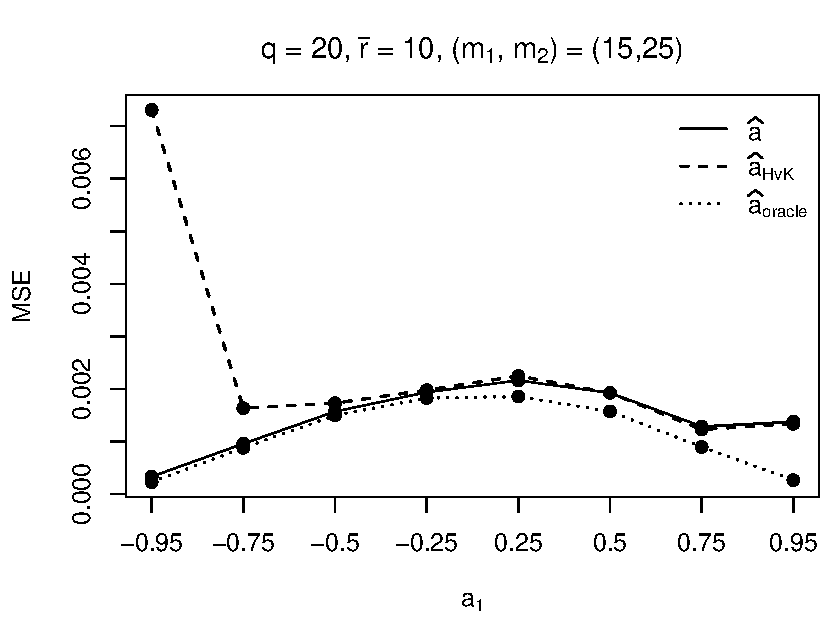
\includegraphics[width=\textwidth]{Plots/Robustness/MSE_a1_T=500_slope=1_(q,r,M1,M2)=(20,10,15,25).pdf}
\end{subfigure}
\hspace{0.25cm}
\begin{subfigure}[b]{0.45\textwidth}
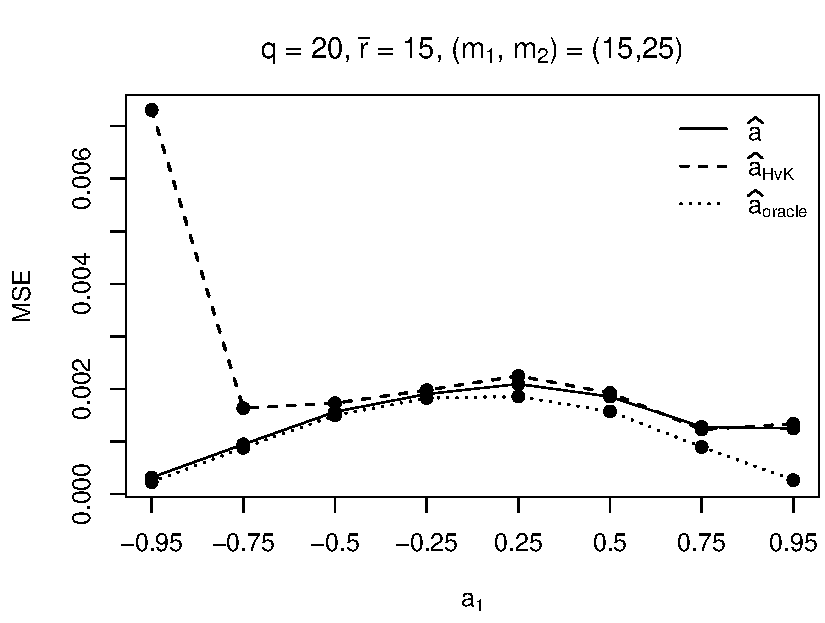
\includegraphics[width=\textwidth]{Plots/Robustness/MSE_a1_T=500_slope=1_(q,r,M1,M2)=(20,15,15,25).pdf}
\end{subfigure}

\begin{subfigure}[b]{0.45\textwidth}
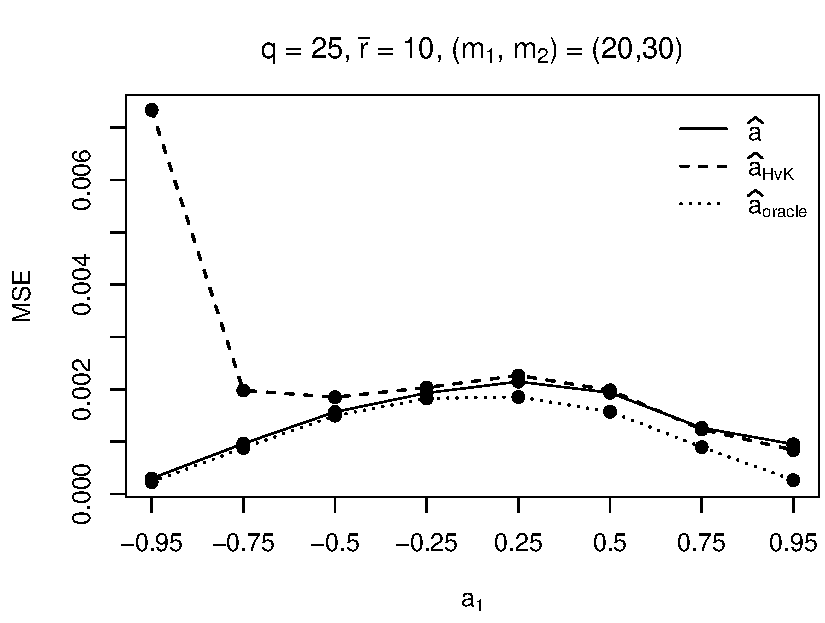
\includegraphics[width=\textwidth]{Plots/Robustness/MSE_a1_T=500_slope=1_(q,r,M1,M2)=(25,10,20,30).pdf}
\end{subfigure}
\hspace{0.25cm}
\begin{subfigure}[b]{0.45\textwidth}
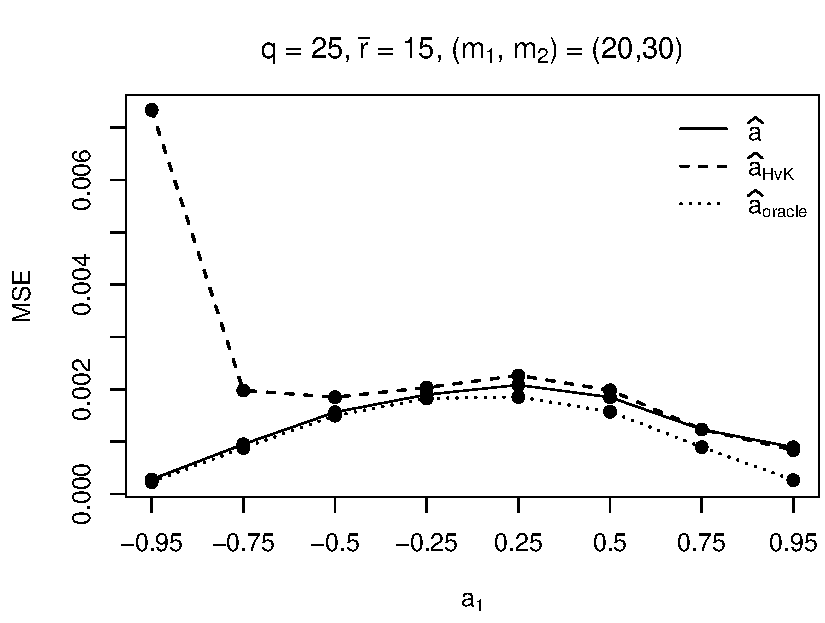
\includegraphics[width=\textwidth]{Plots/Robustness/MSE_a1_T=500_slope=1_(q,r,M1,M2)=(25,15,20,30).pdf}
\end{subfigure}

\begin{subfigure}[b]{0.45\textwidth}
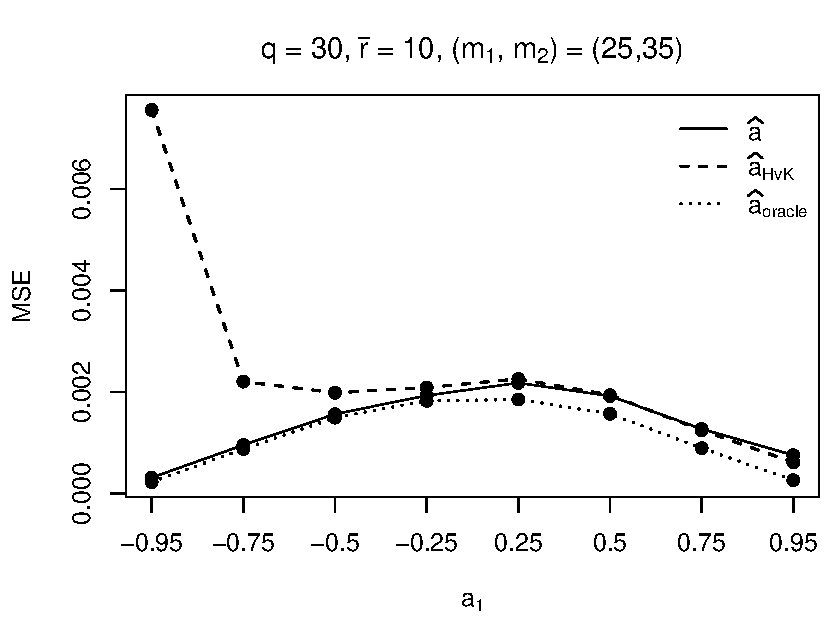
\includegraphics[width=\textwidth]{Plots/Robustness/MSE_a1_T=500_slope=1_(q,r,M1,M2)=(30,10,25,35).pdf}
\end{subfigure}
\hspace{0.25cm}
\begin{subfigure}[b]{0.45\textwidth}
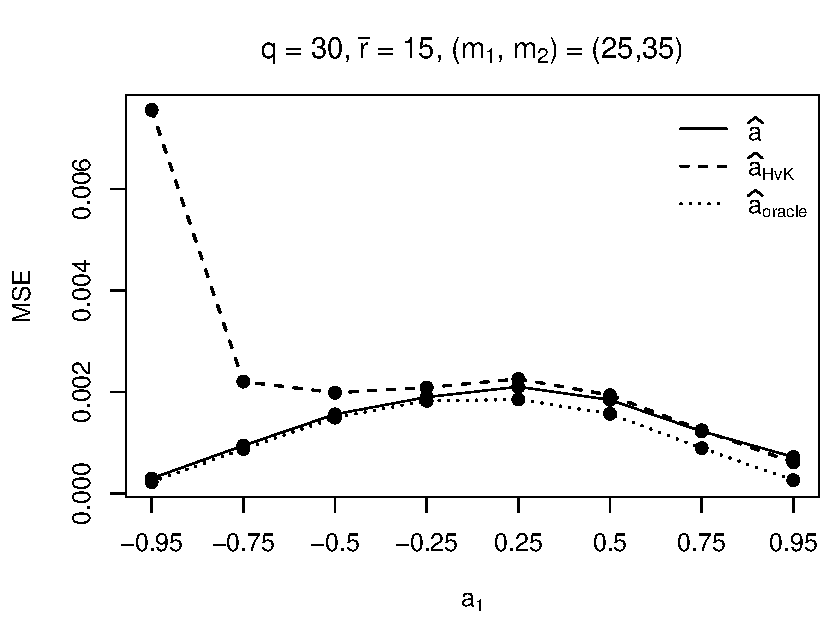
\includegraphics[width=\textwidth]{Plots/Robustness/MSE_a1_T=500_slope=1_(q,r,M1,M2)=(30,15,25,35).pdf}
\end{subfigure}

\begin{subfigure}[b]{0.45\textwidth}
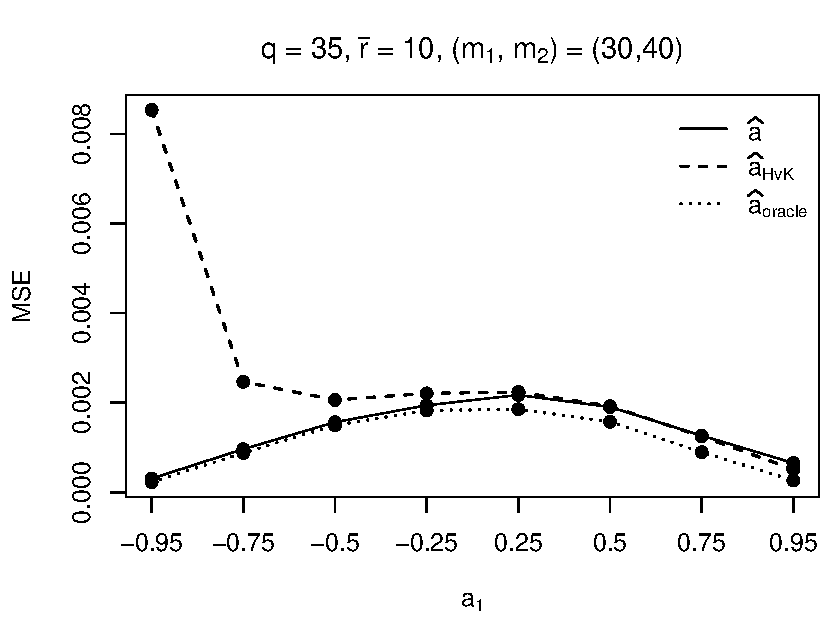
\includegraphics[width=\textwidth]{Plots/Robustness/MSE_a1_T=500_slope=1_(q,r,M1,M2)=(35,10,30,40).pdf}
\end{subfigure}
\hspace{0.25cm}
\begin{subfigure}[b]{0.45\textwidth}
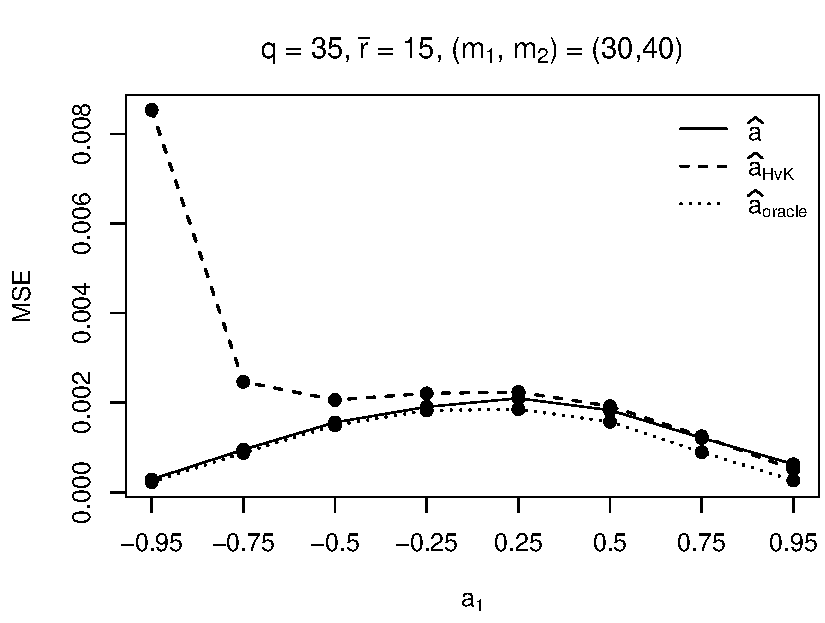
\includegraphics[width=\textwidth]{Plots/Robustness/MSE_a1_T=500_slope=1_(q,r,M1,M2)=(35,15,30,40).pdf}
\end{subfigure}
\caption{MSE values for the estimators $\widehat{a}$, $\widehat{a}_{\text{HvK}}$ and $\widehat{a}_{\text{oracle}}$ in the scenario with a moderate trend ($s_\beta=1$).}\label{fig:MSE_slope1_AR_robust} 
\end{figure}


\begin{figure}[p]
\begin{subfigure}[b]{0.45\textwidth}
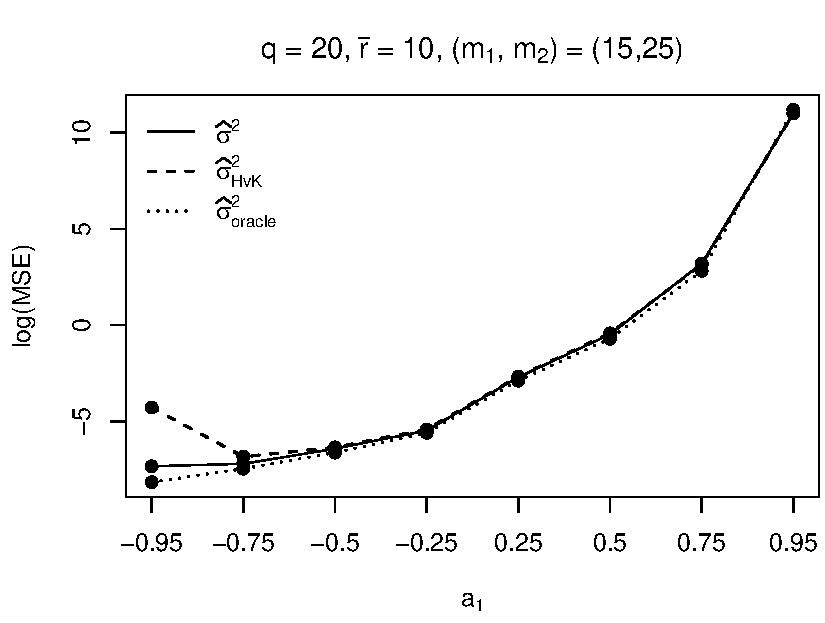
\includegraphics[width=\textwidth]{Plots/Robustness/MSE_lrv_T=500_slope=1_(q,r,M1,M2)=(20,10,15,25).pdf}
\end{subfigure}
\hspace{0.25cm}
\begin{subfigure}[b]{0.45\textwidth}
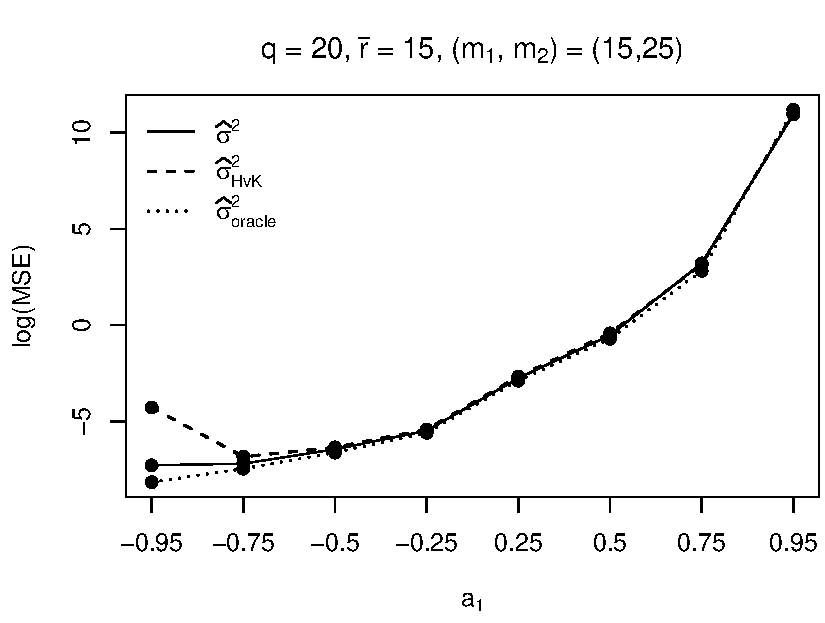
\includegraphics[width=\textwidth]{Plots/Robustness/MSE_lrv_T=500_slope=1_(q,r,M1,M2)=(20,15,15,25).pdf}
\end{subfigure}

\begin{subfigure}[b]{0.45\textwidth}
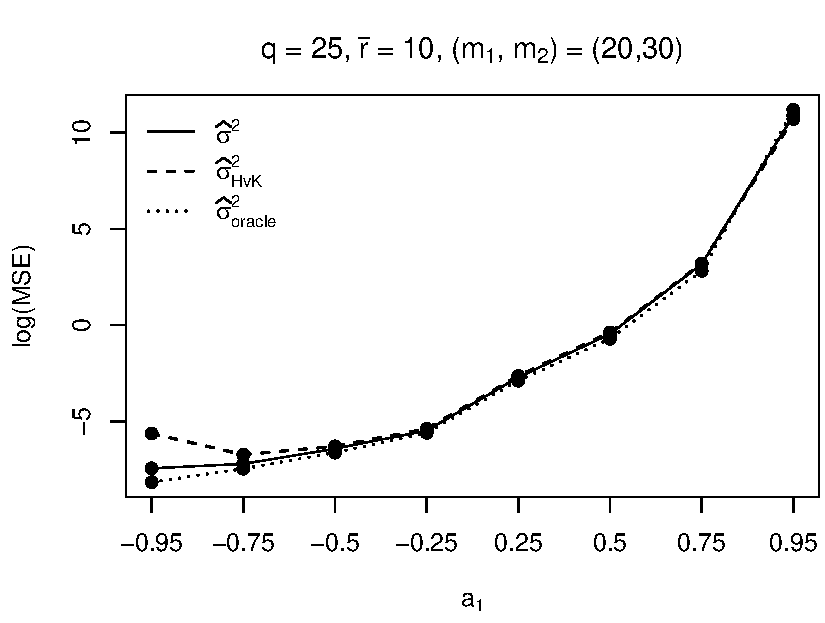
\includegraphics[width=\textwidth]{Plots/Robustness/MSE_lrv_T=500_slope=1_(q,r,M1,M2)=(25,10,20,30).pdf}
\end{subfigure}
\hspace{0.25cm}
\begin{subfigure}[b]{0.45\textwidth}
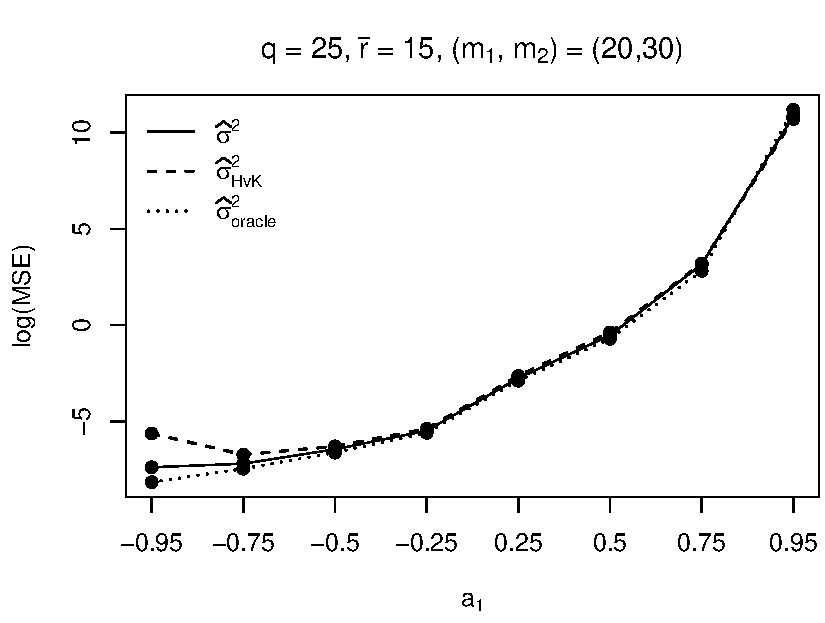
\includegraphics[width=\textwidth]{Plots/Robustness/MSE_lrv_T=500_slope=1_(q,r,M1,M2)=(25,15,20,30).pdf}
\end{subfigure}

\begin{subfigure}[b]{0.45\textwidth}
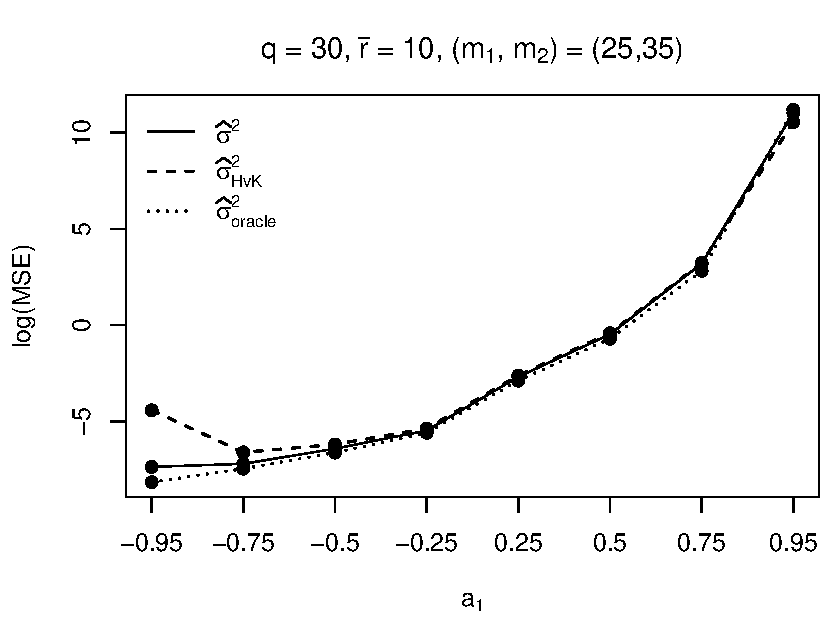
\includegraphics[width=\textwidth]{Plots/Robustness/MSE_lrv_T=500_slope=1_(q,r,M1,M2)=(30,10,25,35).pdf}
\end{subfigure}
\hspace{0.25cm}
\begin{subfigure}[b]{0.45\textwidth}
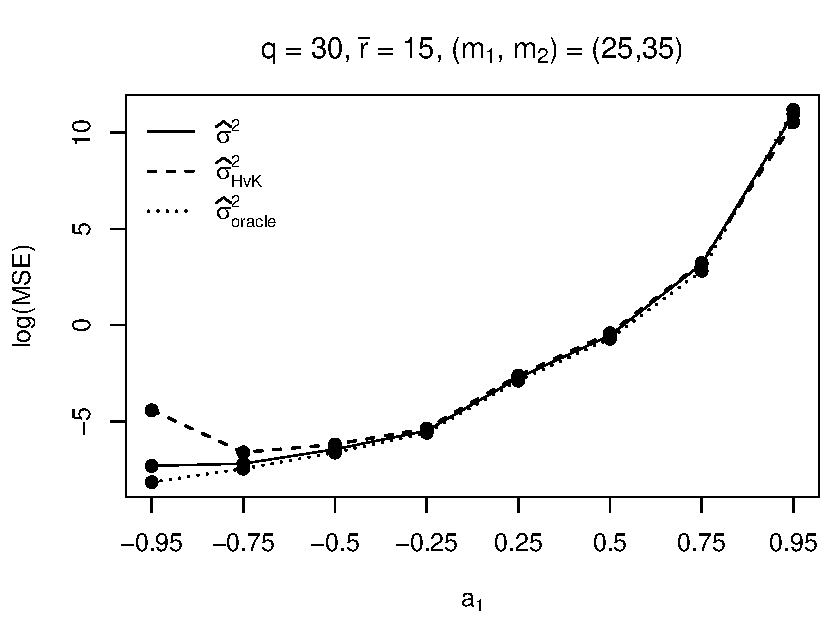
\includegraphics[width=\textwidth]{Plots/Robustness/MSE_lrv_T=500_slope=1_(q,r,M1,M2)=(30,15,25,35).pdf}
\end{subfigure}

\begin{subfigure}[b]{0.45\textwidth}
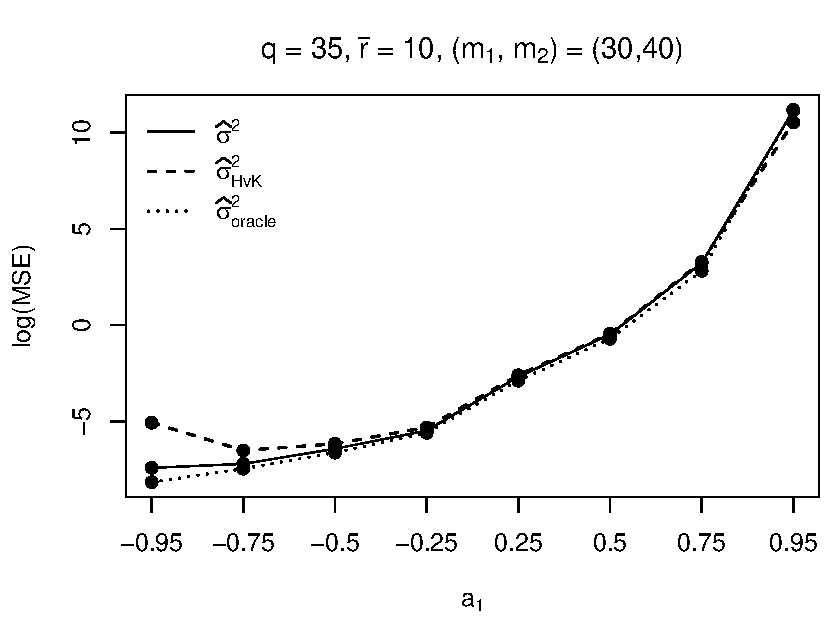
\includegraphics[width=\textwidth]{Plots/Robustness/MSE_lrv_T=500_slope=1_(q,r,M1,M2)=(35,10,30,40).pdf}
\end{subfigure}
\hspace{0.25cm}
\begin{subfigure}[b]{0.45\textwidth}
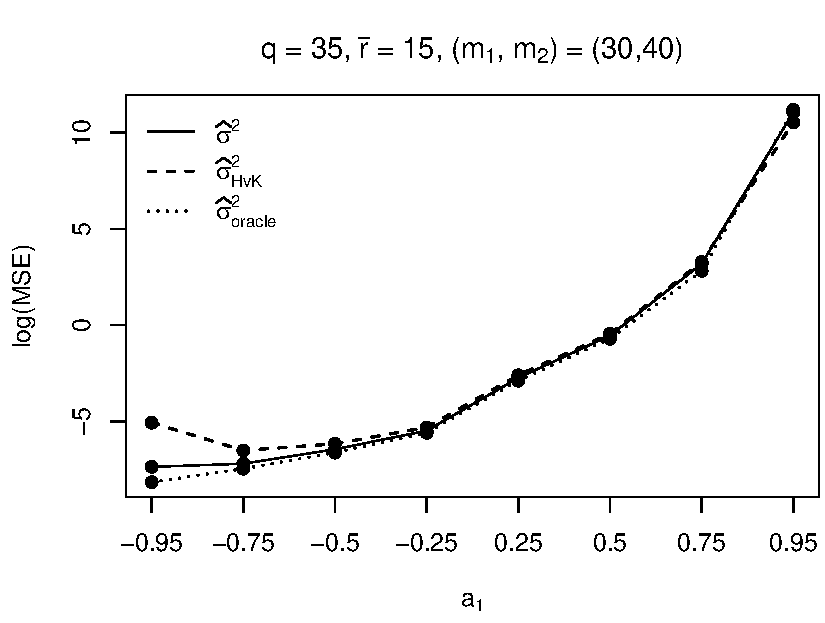
\includegraphics[width=\textwidth]{Plots/Robustness/MSE_lrv_T=500_slope=1_(q,r,M1,M2)=(35,15,30,40).pdf}
\end{subfigure}
\caption{Logarithmic MSE values for the estimators $\widehat{\sigma}^2$, $\widehat{\sigma}^2_{\text{HvK}}$ and $\widehat{\sigma}^2_{\text{oracle}}$ in the scenario with a moderate trend ($s_\beta=1$).}\label{fig:MSE_slope1_lrv_robust}
\end{figure}


\begin{figure}[p]
\begin{subfigure}[b]{0.45\textwidth}
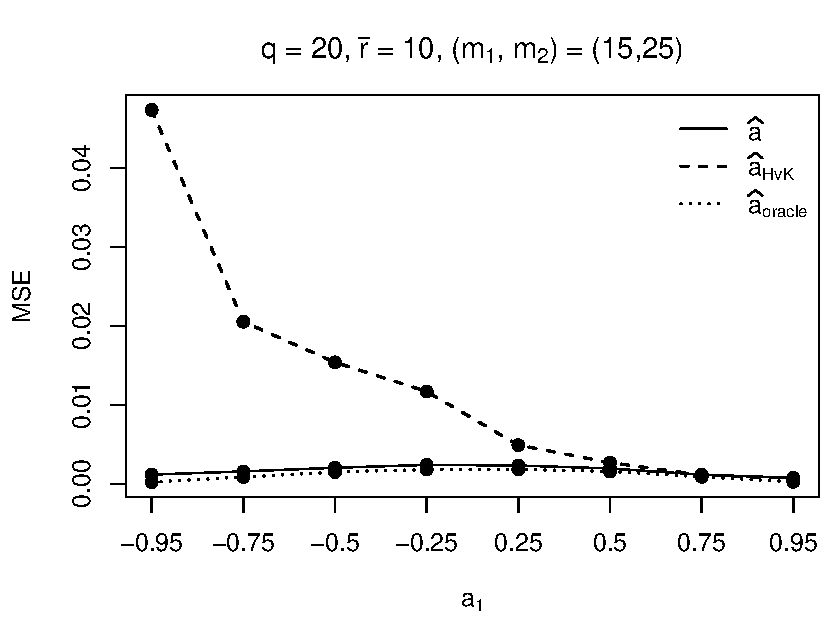
\includegraphics[width=\textwidth]{Plots/Robustness/MSE_a1_T=500_slope=10_(q,r,M1,M2)=(20,10,15,25).pdf}
\end{subfigure}
\hspace{0.25cm}
\begin{subfigure}[b]{0.45\textwidth}
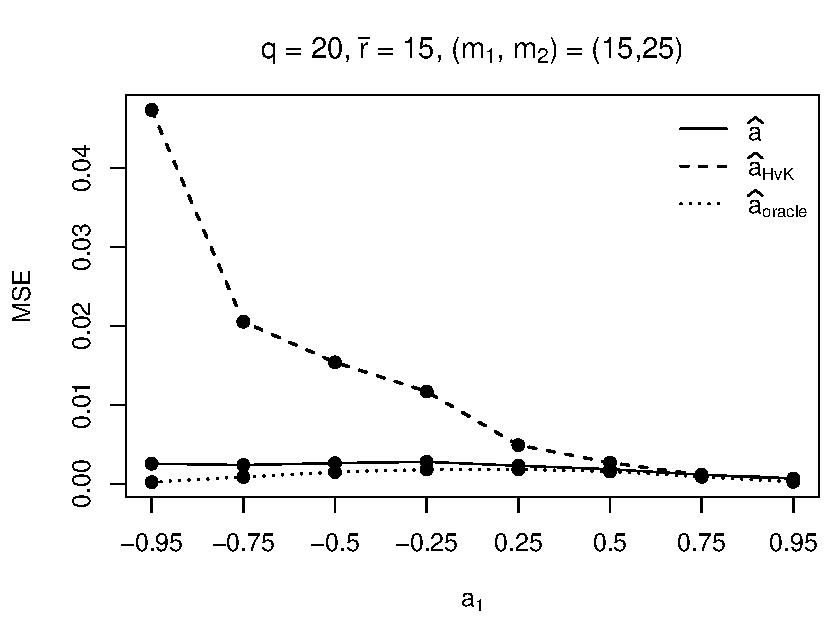
\includegraphics[width=\textwidth]{Plots/Robustness/MSE_a1_T=500_slope=10_(q,r,M1,M2)=(20,15,15,25).pdf}
\end{subfigure}

\begin{subfigure}[b]{0.45\textwidth}
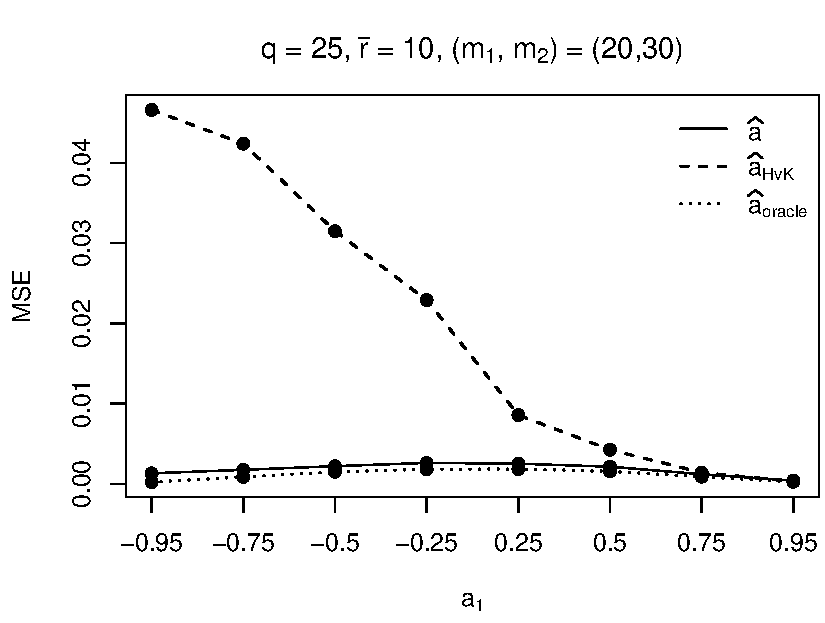
\includegraphics[width=\textwidth]{Plots/Robustness/MSE_a1_T=500_slope=10_(q,r,M1,M2)=(25,10,20,30).pdf}
\end{subfigure}
\hspace{0.25cm}
\begin{subfigure}[b]{0.45\textwidth}
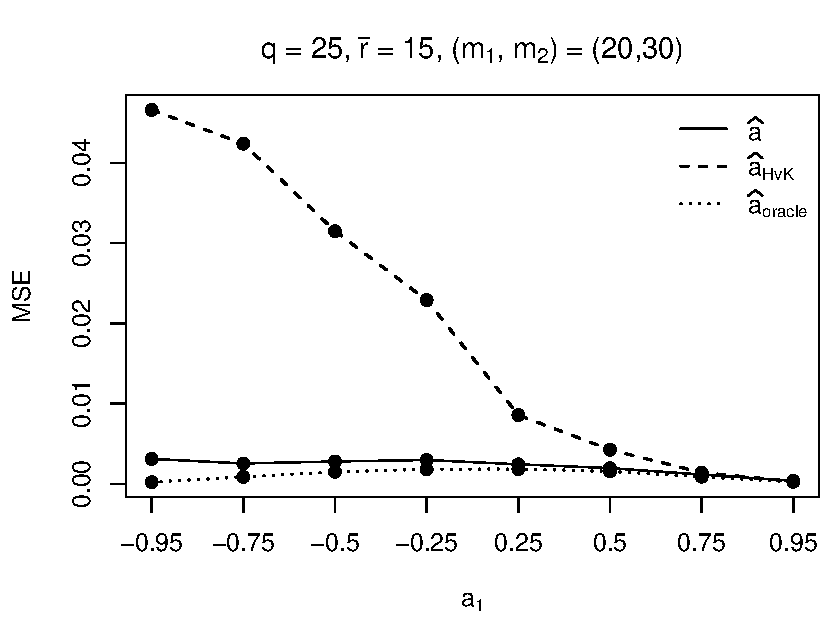
\includegraphics[width=\textwidth]{Plots/Robustness/MSE_a1_T=500_slope=10_(q,r,M1,M2)=(25,15,20,30).pdf}
\end{subfigure}

\begin{subfigure}[b]{0.45\textwidth}
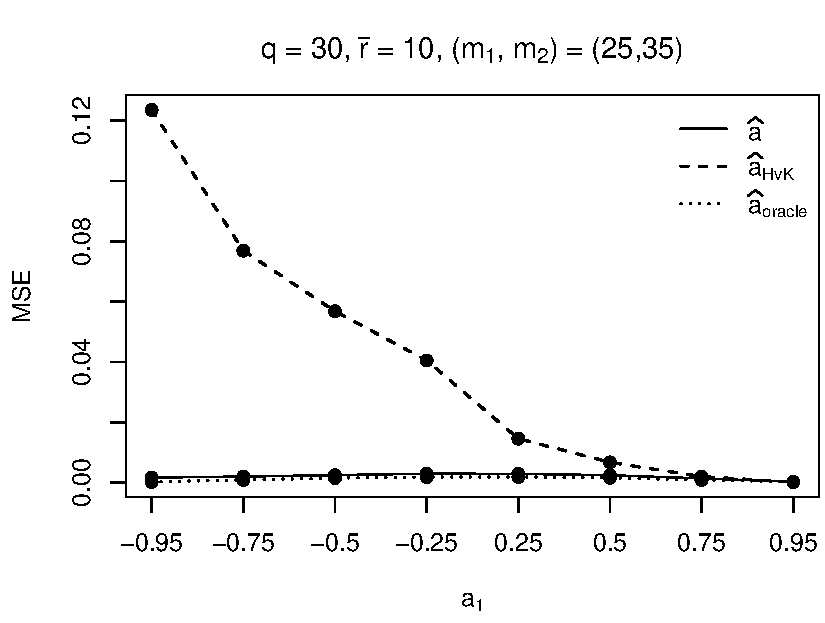
\includegraphics[width=\textwidth]{Plots/Robustness/MSE_a1_T=500_slope=10_(q,r,M1,M2)=(30,10,25,35).pdf}
\end{subfigure}
\hspace{0.25cm}
\begin{subfigure}[b]{0.45\textwidth}
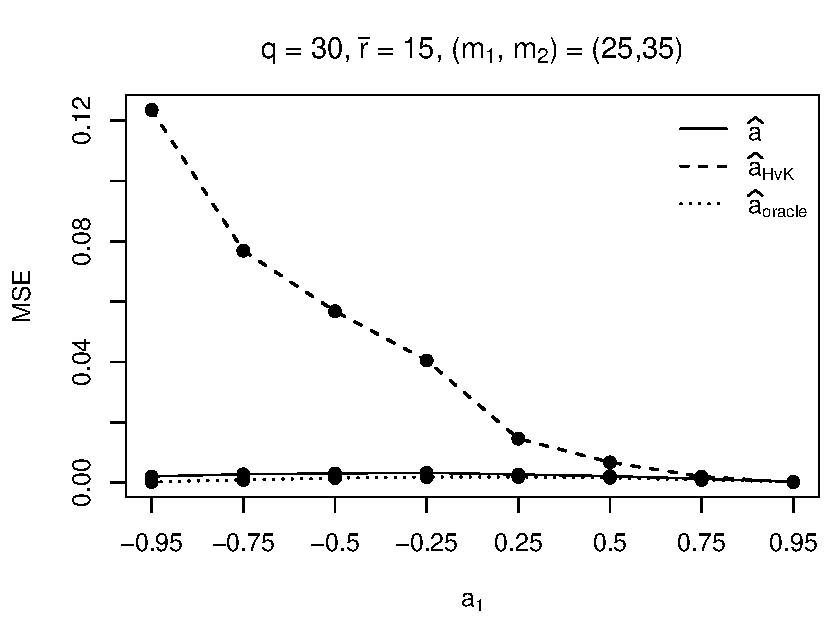
\includegraphics[width=\textwidth]{Plots/Robustness/MSE_a1_T=500_slope=10_(q,r,M1,M2)=(30,15,25,35).pdf}
\end{subfigure}

\begin{subfigure}[b]{0.45\textwidth}
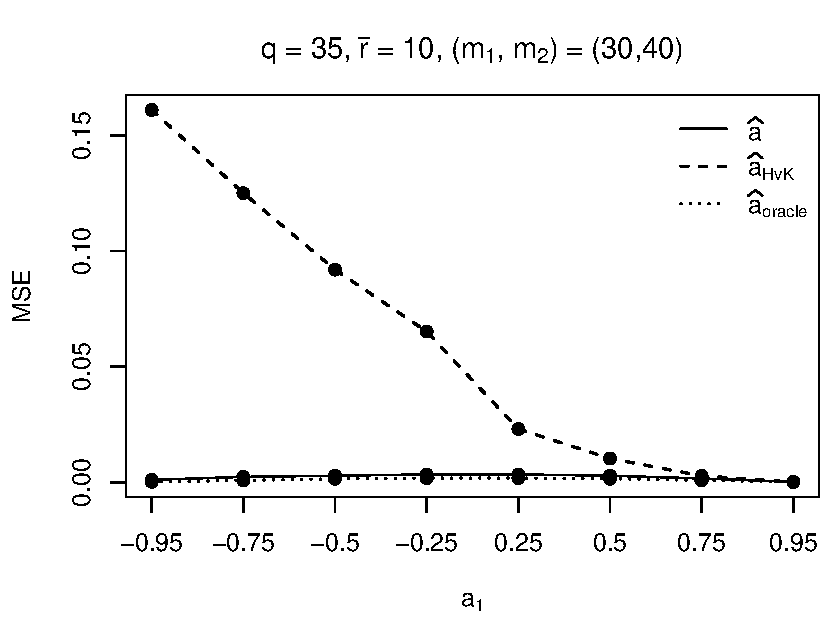
\includegraphics[width=\textwidth]{Plots/Robustness/MSE_a1_T=500_slope=10_(q,r,M1,M2)=(35,10,30,40).pdf}
\end{subfigure}
\hspace{0.25cm}
\begin{subfigure}[b]{0.45\textwidth}
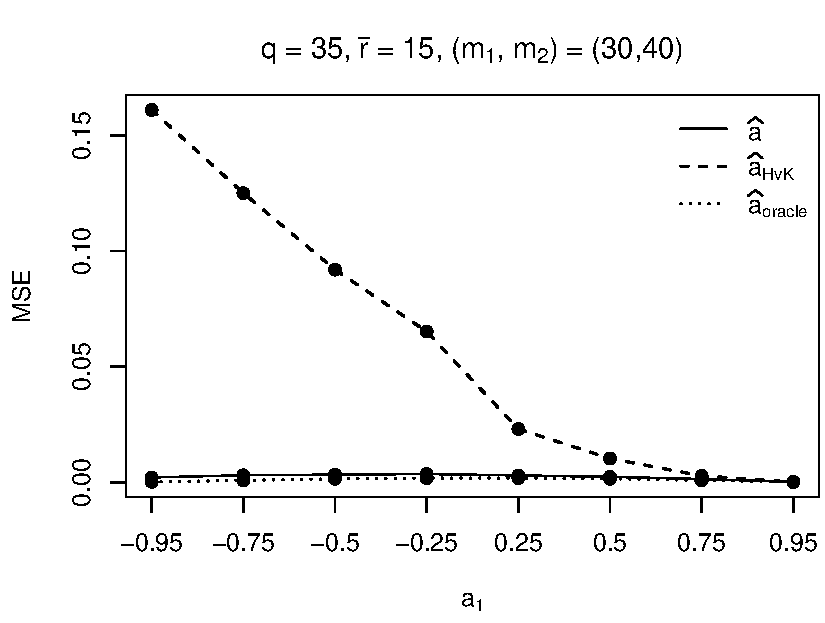
\includegraphics[width=\textwidth]{Plots/Robustness/MSE_a1_T=500_slope=10_(q,r,M1,M2)=(35,15,30,40).pdf}
\end{subfigure}
\caption{MSE values for the estimators $\widehat{a}$, $\widehat{a}_{\text{HvK}}$ and $\widehat{a}_{\text{oracle}}$ in the scenario with a pronounced trend ($s_\beta=10$).}\label{fig:MSE_slope10_AR_robust} 
\end{figure}


\begin{figure}[p]
\begin{subfigure}[b]{0.45\textwidth}
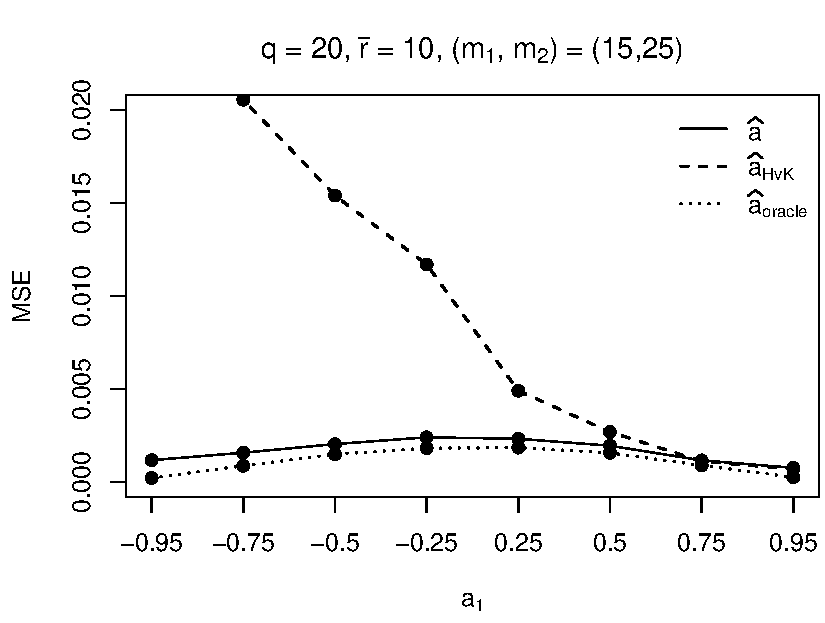
\includegraphics[width=\textwidth]{Plots/Robustness/MSE_a1_zoomed_T=500_slope=10_(q,r,M1,M2)=(20,10,15,25).pdf}
\end{subfigure}
\hspace{0.25cm}
\begin{subfigure}[b]{0.45\textwidth}
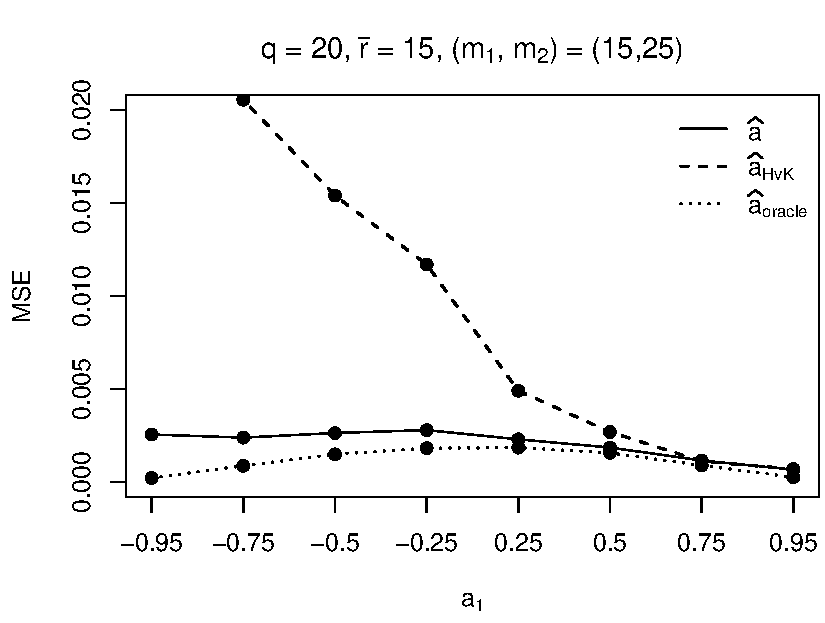
\includegraphics[width=\textwidth]{Plots/Robustness/MSE_a1_zoomed_T=500_slope=10_(q,r,M1,M2)=(20,15,15,25).pdf}
\end{subfigure}

\begin{subfigure}[b]{0.45\textwidth}
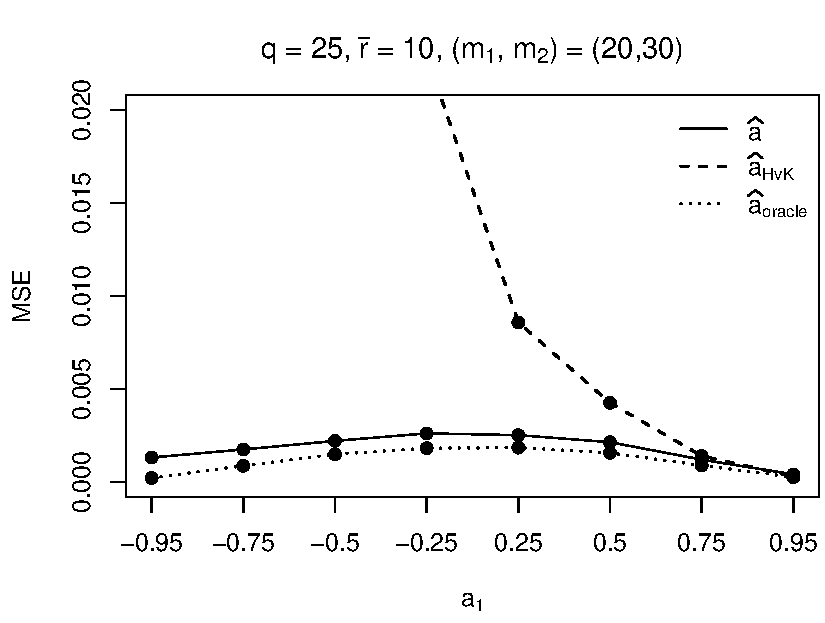
\includegraphics[width=\textwidth]{Plots/Robustness/MSE_a1_zoomed_T=500_slope=10_(q,r,M1,M2)=(25,10,20,30).pdf}
\end{subfigure}
\hspace{0.25cm}
\begin{subfigure}[b]{0.45\textwidth}
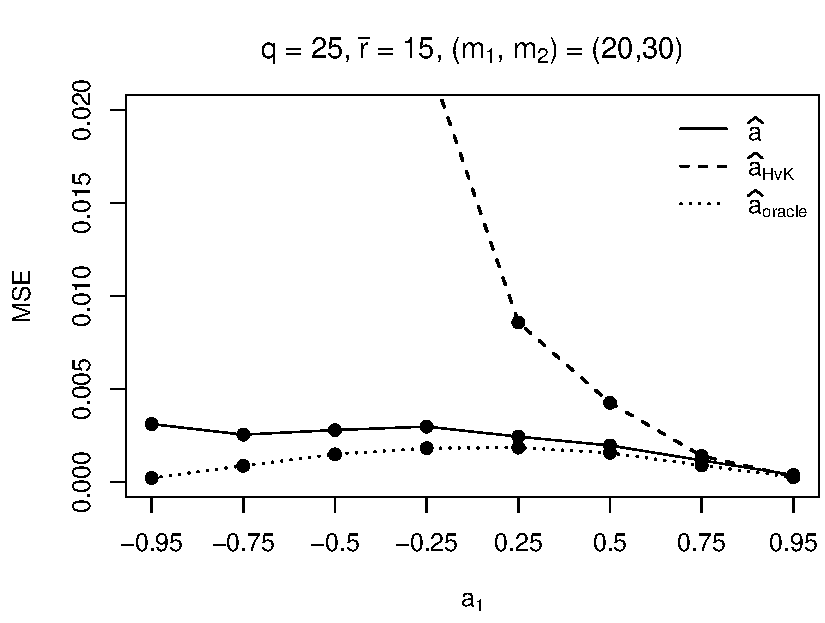
\includegraphics[width=\textwidth]{Plots/Robustness/MSE_a1_zoomed_T=500_slope=10_(q,r,M1,M2)=(25,15,20,30).pdf}
\end{subfigure}

\begin{subfigure}[b]{0.45\textwidth}
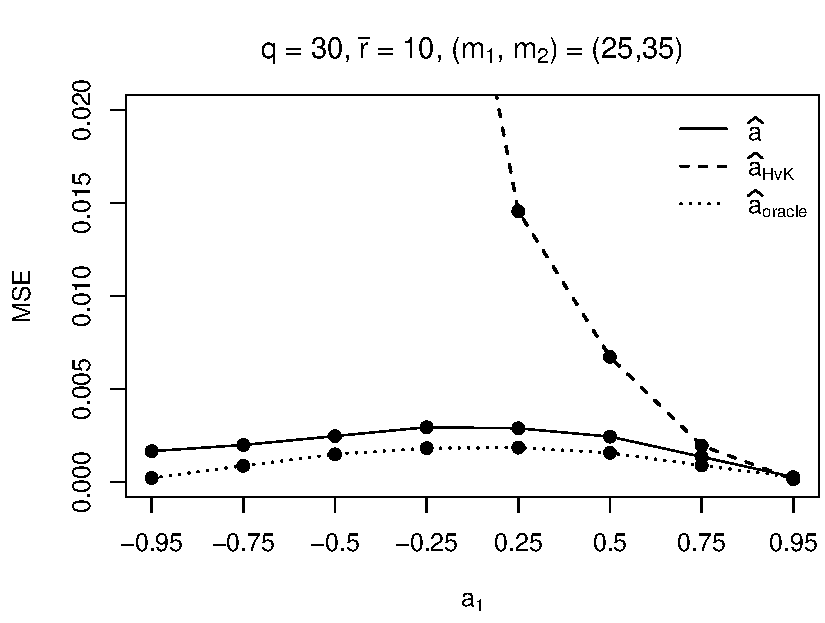
\includegraphics[width=\textwidth]{Plots/Robustness/MSE_a1_zoomed_T=500_slope=10_(q,r,M1,M2)=(30,10,25,35).pdf}
\end{subfigure}
\hspace{0.25cm}
\begin{subfigure}[b]{0.45\textwidth}
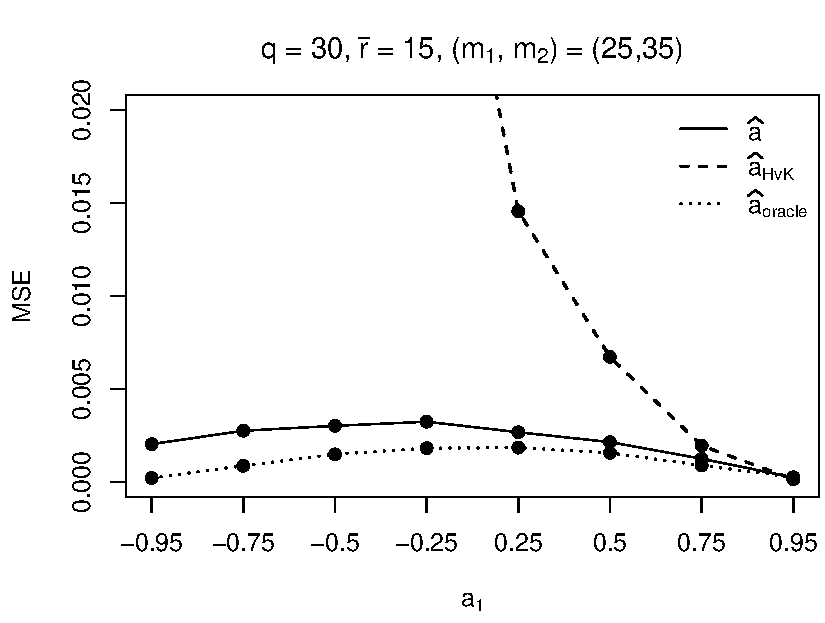
\includegraphics[width=\textwidth]{Plots/Robustness/MSE_a1_zoomed_T=500_slope=10_(q,r,M1,M2)=(30,15,25,35).pdf}
\end{subfigure}

\begin{subfigure}[b]{0.45\textwidth}
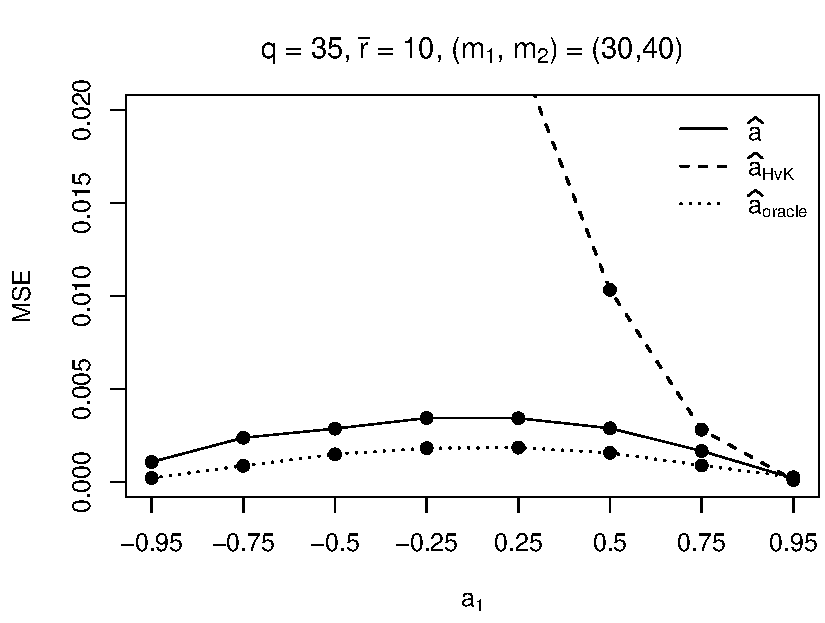
\includegraphics[width=\textwidth]{Plots/Robustness/MSE_a1_zoomed_T=500_slope=10_(q,r,M1,M2)=(35,10,30,40).pdf}
\end{subfigure}
\hspace{0.25cm}
\begin{subfigure}[b]{0.45\textwidth}
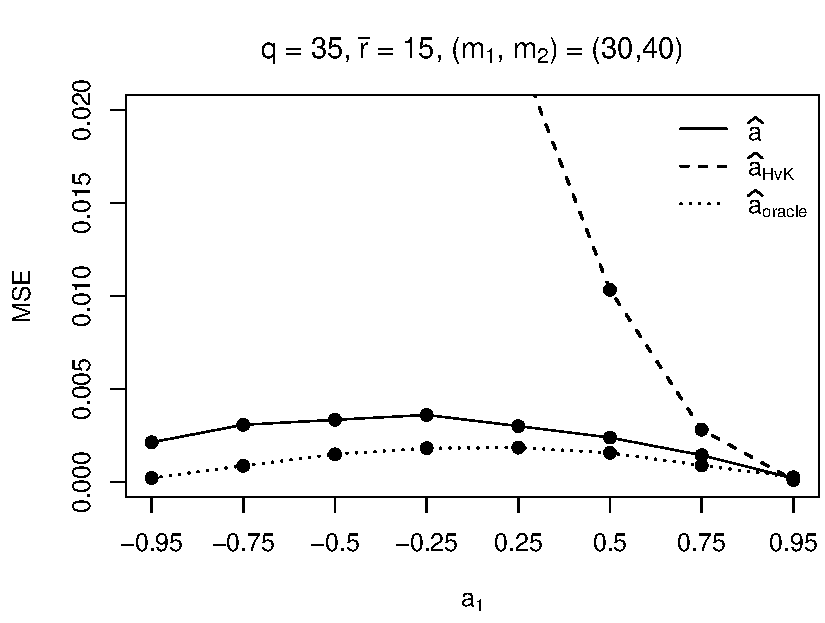
\includegraphics[width=\textwidth]{Plots/Robustness/MSE_a1_zoomed_T=500_slope=10_(q,r,M1,M2)=(35,15,30,40).pdf}
\end{subfigure}
\caption{MSE values for the estimators $\widehat{a}$, $\widehat{a}_{\text{HvK}}$ and $\widehat{a}_{\text{oracle}}$ in the scenario with a pronounced trend ($s_\beta=10$). The plots are zoomed-in versions of the respective plots in Figure \ref{fig:MSE_slope10_AR_robust}.}\label{fig:MSE_slope10_AR_zoom_robust}
\end{figure}


\begin{figure}[p]
\begin{subfigure}[b]{0.45\textwidth}
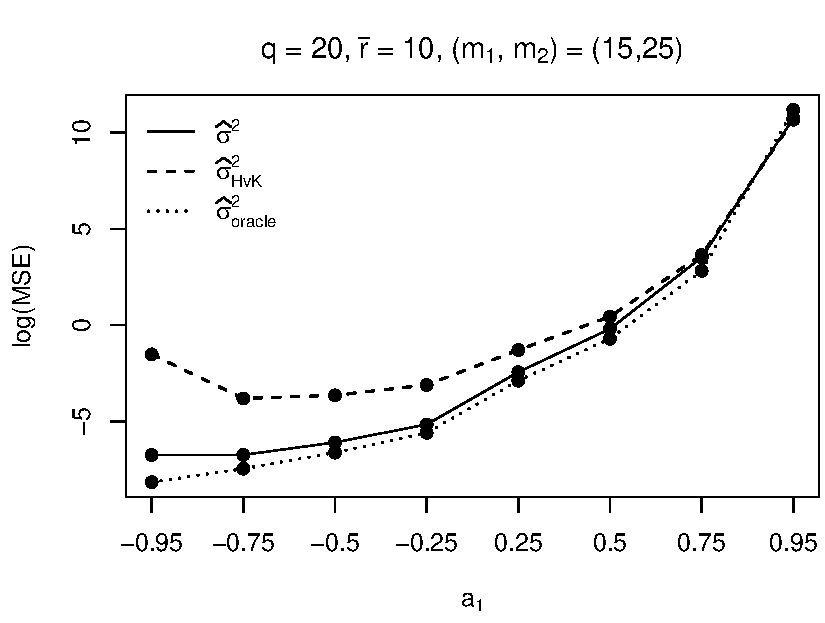
\includegraphics[width=\textwidth]{Plots/Robustness/MSE_lrv_T=500_slope=10_(q,r,M1,M2)=(20,10,15,25).pdf}
\end{subfigure}
\hspace{0.25cm}
\begin{subfigure}[b]{0.45\textwidth}
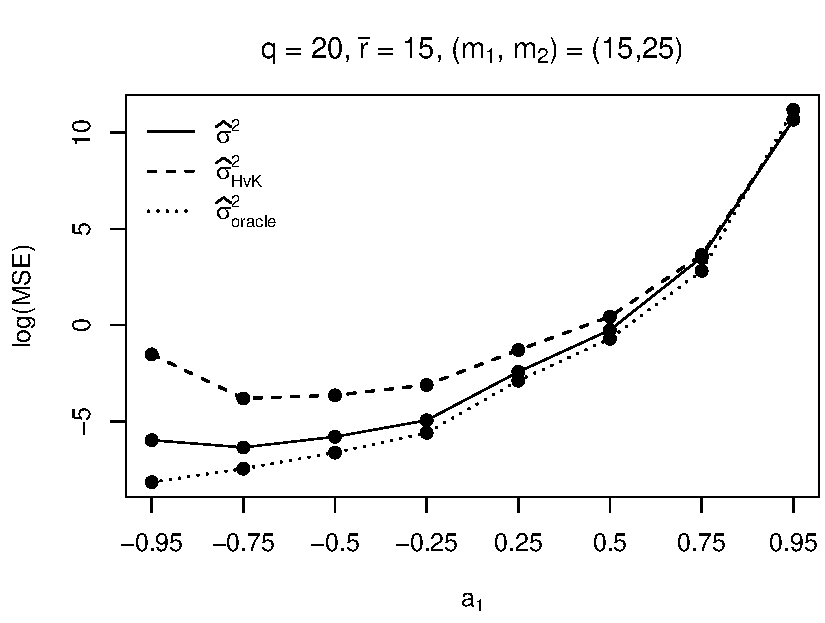
\includegraphics[width=\textwidth]{Plots/Robustness/MSE_lrv_T=500_slope=10_(q,r,M1,M2)=(20,15,15,25).pdf}
\end{subfigure}

\begin{subfigure}[b]{0.45\textwidth}
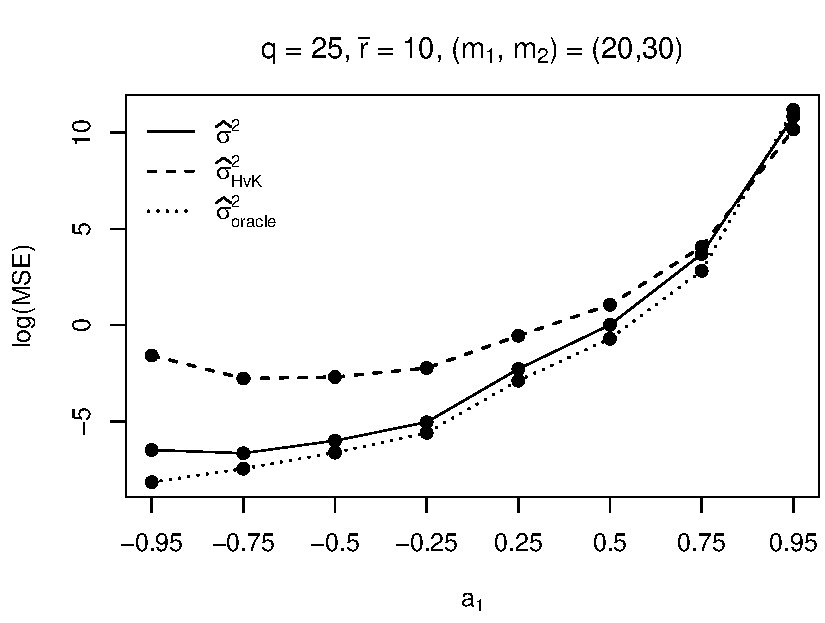
\includegraphics[width=\textwidth]{Plots/Robustness/MSE_lrv_T=500_slope=10_(q,r,M1,M2)=(25,10,20,30).pdf}
\end{subfigure}
\hspace{0.25cm}
\begin{subfigure}[b]{0.45\textwidth}
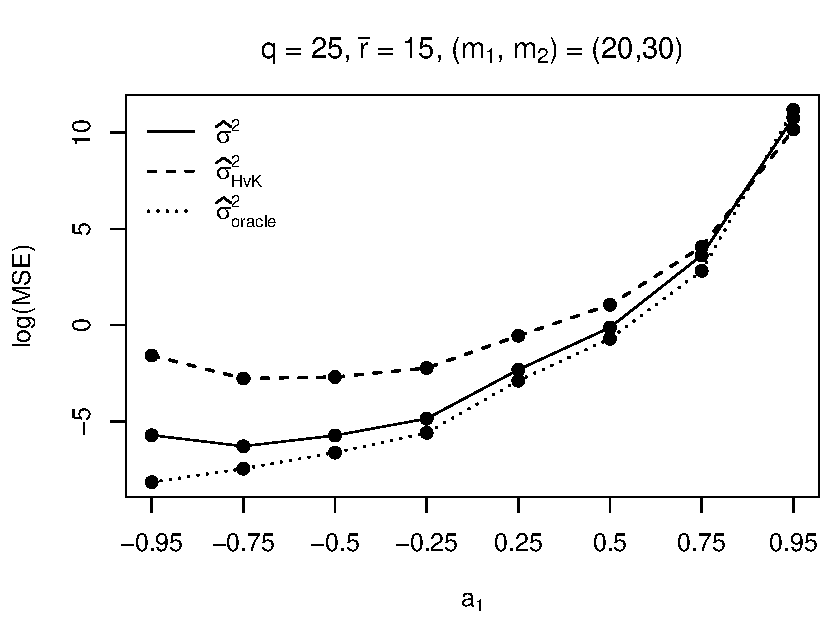
\includegraphics[width=\textwidth]{Plots/Robustness/MSE_lrv_T=500_slope=10_(q,r,M1,M2)=(25,15,20,30).pdf}
\end{subfigure}

\begin{subfigure}[b]{0.45\textwidth}
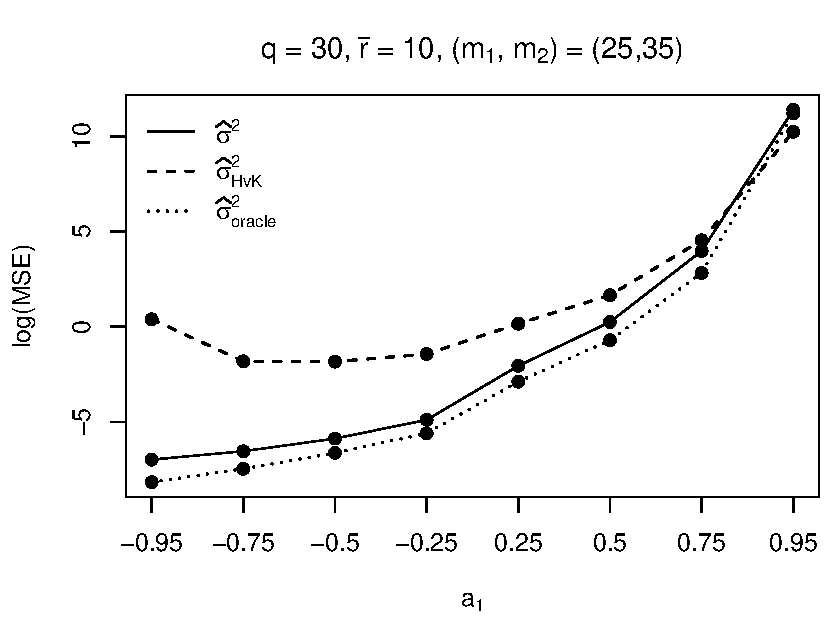
\includegraphics[width=\textwidth]{Plots/Robustness/MSE_lrv_T=500_slope=10_(q,r,M1,M2)=(30,10,25,35).pdf}
\end{subfigure}
\hspace{0.25cm}
\begin{subfigure}[b]{0.45\textwidth}
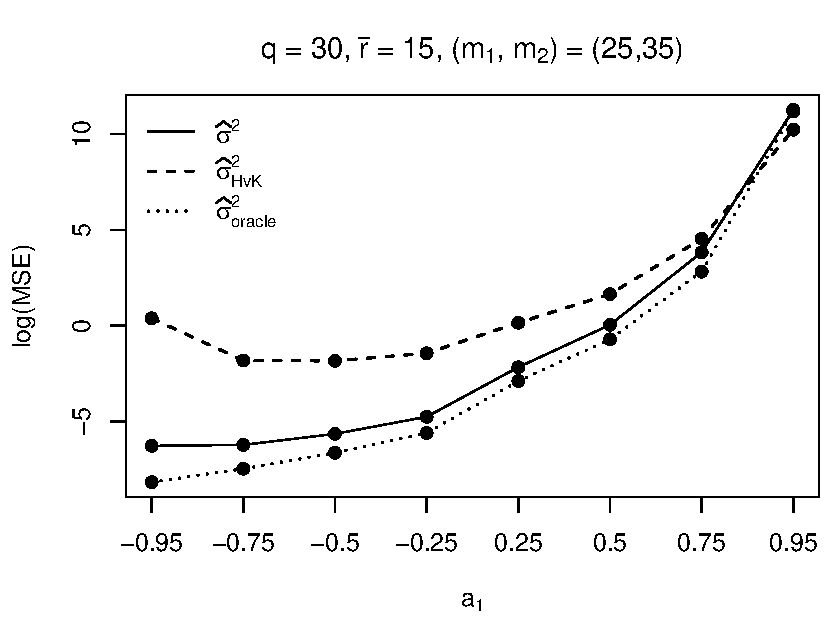
\includegraphics[width=\textwidth]{Plots/Robustness/MSE_lrv_T=500_slope=10_(q,r,M1,M2)=(30,15,25,35).pdf}
\end{subfigure}

\begin{subfigure}[b]{0.45\textwidth}
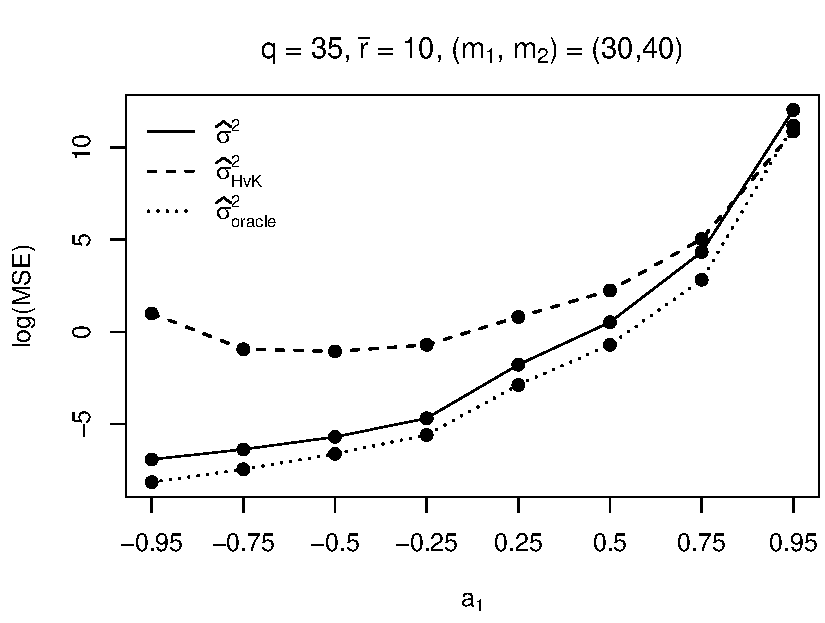
\includegraphics[width=\textwidth]{Plots/Robustness/MSE_lrv_T=500_slope=10_(q,r,M1,M2)=(35,10,30,40).pdf}
\end{subfigure}
\hspace{0.25cm}
\begin{subfigure}[b]{0.45\textwidth}
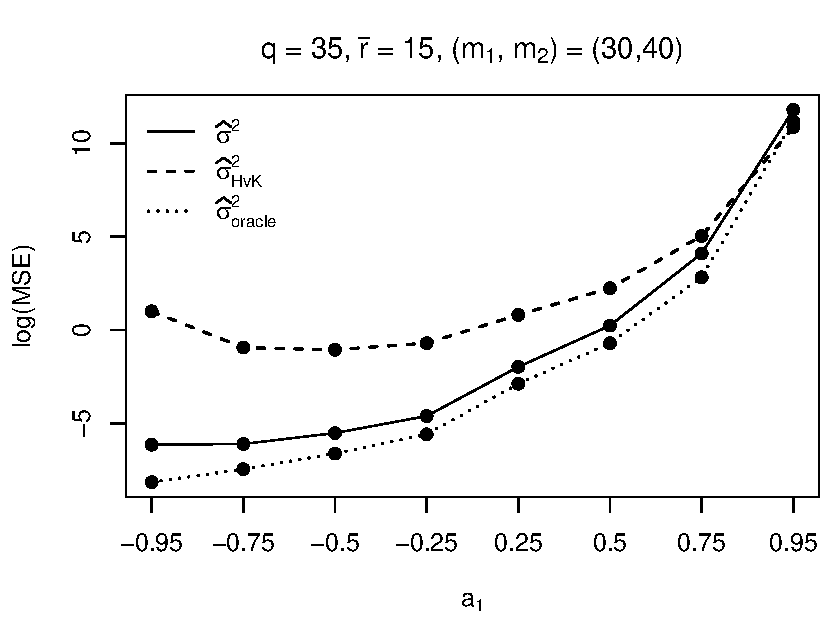
\includegraphics[width=\textwidth]{Plots/Robustness/MSE_lrv_T=500_slope=10_(q,r,M1,M2)=(35,15,30,40).pdf}
\end{subfigure}
\caption{Logarithmic MSE values for the estimators $\widehat{\sigma}^2$, $\widehat{\sigma}^2_{\text{HvK}}$ and $\widehat{\sigma}^2_{\text{oracle}}$ in the scenario with a pronounced trend ($s_\beta=10$).}\label{fig:MSE_slope10_lrv_robust} 
\end{figure}


\FloatBarrier
\newpage
\subsection*{Implementation of SiZer in Section \ref{subsec-sim-2}}


The SiZer methods for the comparison study in Section \ref{subsec-sim-2} are implemented as follows:
\begin{enumerate}[leftmargin=0.7cm,label=(\alph*)]

\item Computation of the grid $\mathcal{G}_T^*$:

To start with, we compute the variance of $\bar{Y} = T^{-1} \sum_{t=1}^T Y_{t,T}$, which is given by
\[ \var(\bar{Y}) = \frac{\gamma_\varepsilon(0)}{T} + \frac{2}{T} \sum_{k = 1}^{T-1} \Big(1 - \frac{k}{T}\Big)\gamma_\varepsilon(k). \]
Since the autocovariance function $\gamma_{\varepsilon}(\cdot)$ is known by assumption, we can calculate the value of $\var(\bar{Y})$ by using the formula $\gamma_\varepsilon(k) = \nu^2 a_1^{|k|} / (1 - a_1^2)$ together with the true para\-meters $a_1$ and $\nu^2 = \ex[\eta_t^2]$. We next compute 
\[ T^* = \frac{\gamma_\varepsilon(0)}{\var(\bar{Y})}, \]
which can be interpreted as a measure of information in the data. For each point $(u,h) \in \mathcal{G}_T$ from \eqref{grid-sim-app}, we finally calculate the effective sample size for dependent data 
\[ \text{ESS}^*(u, h) = \frac{T^*}{T} \frac{\sum_{t=1}^T K_h(t/T - u)}{K_h(0)} \]
with $K_h(v) = h^{-1} K(v/h)$ and set $\mathcal{G}_T^* = \{ (u,h) \in \mathcal{G}_T: \text{ESS}^*(u, h) \ge 5 \}$. 

\item Computation of the local linear estimators and their standard deviations: 

For each $(u,h) \in \mathcal{G}_T^*$, we compute a standard local linear estimator $\widehat{m}^\prime_h(u)$ of the derivative $m^\prime(u)$ together with its standard deviation $\text{sd}(\widehat{m}^\prime_h(u))$. The latter is given by $\text{sd}(\widehat{m}^\prime_h(u)) = \{ \var(\widehat{m}^\prime_h(u)) \}^{1/2}$, where $\var(\widehat{m}^\prime_h(u)) = e^\top V e$ with $e = (\begin{matrix} 0 & 1 \end{matrix})^\top$ and 
\[ V = (X^T W X)^{-1} (X^T \Sigma X) (X^T W X)^{-1}. \]
The matrices $X$, $W$ and $\Sigma$ are defined as follows: $\Sigma$ is a $T \times T$ matrix with the elements
\[ \Sigma_{st} = \gamma_\varepsilon(s-t) K_h\Big( \frac{s}{T} - u \Big) K_h\Big( \frac{t}{T} - u \Big), \]
$W$ is a $T \times T$ diagonal matrix with the diagonal entries $K_h(t/T-u)$ and 
\[ X =   
\begin{pmatrix}
1 & (1/T - u)   \\
1 & (2/T - u)   \\
\vdots & \vdots \\
1 & (1 - u)     \\
\end{pmatrix}. \]

\newpage
\item Computation of the confidence intervals:  

For a given confidence level $\alpha$ and for each bandwidth value $h$ with $(u,h) \in \mathcal{G}_T^*$, we compute the quantile 
\[ q(h) = \Phi^{-1} \Big( \Big( 1 - \frac{\alpha}{2} \Big)^{1/(\theta g)} \Big), \]
where $\Phi$ is the distribution function of a standard normal random variable, $g$ is the number of locations $u$ in the grid $\mathcal{G}_T$, and the cluster index $\theta$ is defined on p.1519 in \cite{ParkHannigKang2009}. The confidence interval of $\widehat{m}^\prime_h(u)$ is then computed as $[\widehat{m}^\prime_h(u) - q(h) \, \text{sd}(\widehat{m}^\prime_h(u)),\widehat{m}^\prime_h(u) + q(h) \, \text{sd}(\widehat{m}^\prime_h(u))]$. 

%For each $(u,h) \in \mathcal{G}_T^*$, we compute the Gaussian quantile for the confidence level $\alpha$
%\[ q(u,h) = \Phi^{-1} \Big(\frac{1 + (1 - \alpha)^{\frac{1}{l(u, h)}}}{2}\Big), \]
%where $l(u,h) = T/\text{ESS}^*(u, h)$ and $\Phi$ is the distribution function of a standard normal random variable. The confidence interval of $\widehat{m}^\prime_h(u)$ is then computed as $[\widehat{m}^\prime_h(u) - q(u,h) \, \text{sd}(\widehat{m}^\prime_h(u)),\widehat{m}^\prime_h(u) + q(u,h) \, \text{sd}(\widehat{m}^\prime_h(u))]$. 

\end{enumerate}




\bibliographystyle{ims}
{\small
\setlength{\bibsep}{0.55em}
\bibliography{bibliography}}



\end{document}
